\documentclass[aspectratio=169]{beamer}

% Theme and appearance
\usetheme{Madrid}
\usecolortheme{default}

% Packages
\usepackage[utf8]{inputenc}
\usepackage[T1]{fontenc}
\usepackage{amsmath}
\usepackage{amsfonts}
\usepackage{amssymb}
\usepackage{graphicx}
\usepackage{booktabs}
\usepackage{tikz}
\usepackage{pgfplots}
\pgfplotsset{compat=1.18}
\usepackage{algorithm}
\usepackage{algorithmic}
\usepackage{hyperref}
\usepackage{subcaption}
\usepackage{multirow}
\usepackage{adjustbox}

% TikZ libraries
\usetikzlibrary{shapes,arrows,positioning,calc}

% Colors
\definecolor{berkeleyblue}{RGB}{0,50,98}
\definecolor{berkeleygold}{RGB}{253,181,21}
\definecolor{accent}{RGB}{255,107,107}

% Custom colors for the presentation
\setbeamercolor{structure}{fg=berkeleyblue}
\setbeamercolor{frametitle}{bg=berkeleyblue,fg=white}
\setbeamercolor{title}{fg=berkeleyblue}

% Presentation information
\title[Legal NLP Explainability]{Explainable AI for Legal Document Analysis: \\
A Multi-Method Approach to Clause Extraction}

\subtitle{W266 Final Project Presentation}

\author[Gabriel]{Perry Gabriel}

\institute[UC Berkeley]{
  School of Information \\
  University of California, Berkeley
}

\date{\today}

% Logo (uncomment and adjust path if you have a logo)
% \logo{\includegraphics[height=0.8cm]{../assets/berkeley_logo.png}}

% Footer customization
\setbeamertemplate{footline}[frame number]

% Remove navigation symbols
\setbeamertemplate{navigation symbols}{}

% Custom commands
\newcommand{\highlight}[1]{\textcolor{accent}{\textbf{#1}}}
\newcommand{\figpath}{../../visualizations/figures}

% Document begins
\begin{document}

% Title slide
\frame{\titlepage}

% Outline slide
\begin{frame}{Outline}
\tableofcontents
\end{frame}

% Include sections
% Introduction Section

\section{Introduction}

\begin{frame}{Problem Statement}
\begin{itemize}
    \item \highlight{Legal document analysis} is crucial for contract review and compliance
    \item Traditional manual review is \highlight{time-consuming and error-prone}
    \item NLP models provide automation but lack \highlight{interpretability}
    \item Legal professionals need to understand \highlight{why} AI makes decisions
\end{itemize}

\vspace{0.5cm}
\begin{alertblock}{Research Question}
How can we develop explainable AI methods for automated legal clause extraction that provide interpretable insights for legal professionals?
\end{alertblock}
\end{frame}

\begin{frame}{Motivation}
\begin{columns}
\begin{column}{0.6\textwidth}
\textbf{Why Explainable AI in Legal Domain?}
\begin{itemize}
    \item \highlight{Regulatory compliance} requirements
    \item \highlight{Trust and transparency} for legal professionals
    \item \highlight{Error detection} and model debugging
    \item \highlight{Knowledge discovery} from legal patterns
\end{itemize}
\end{column}
\begin{column}{0.4\textwidth}
\begin{center}
% Show system architecture instead of placeholder
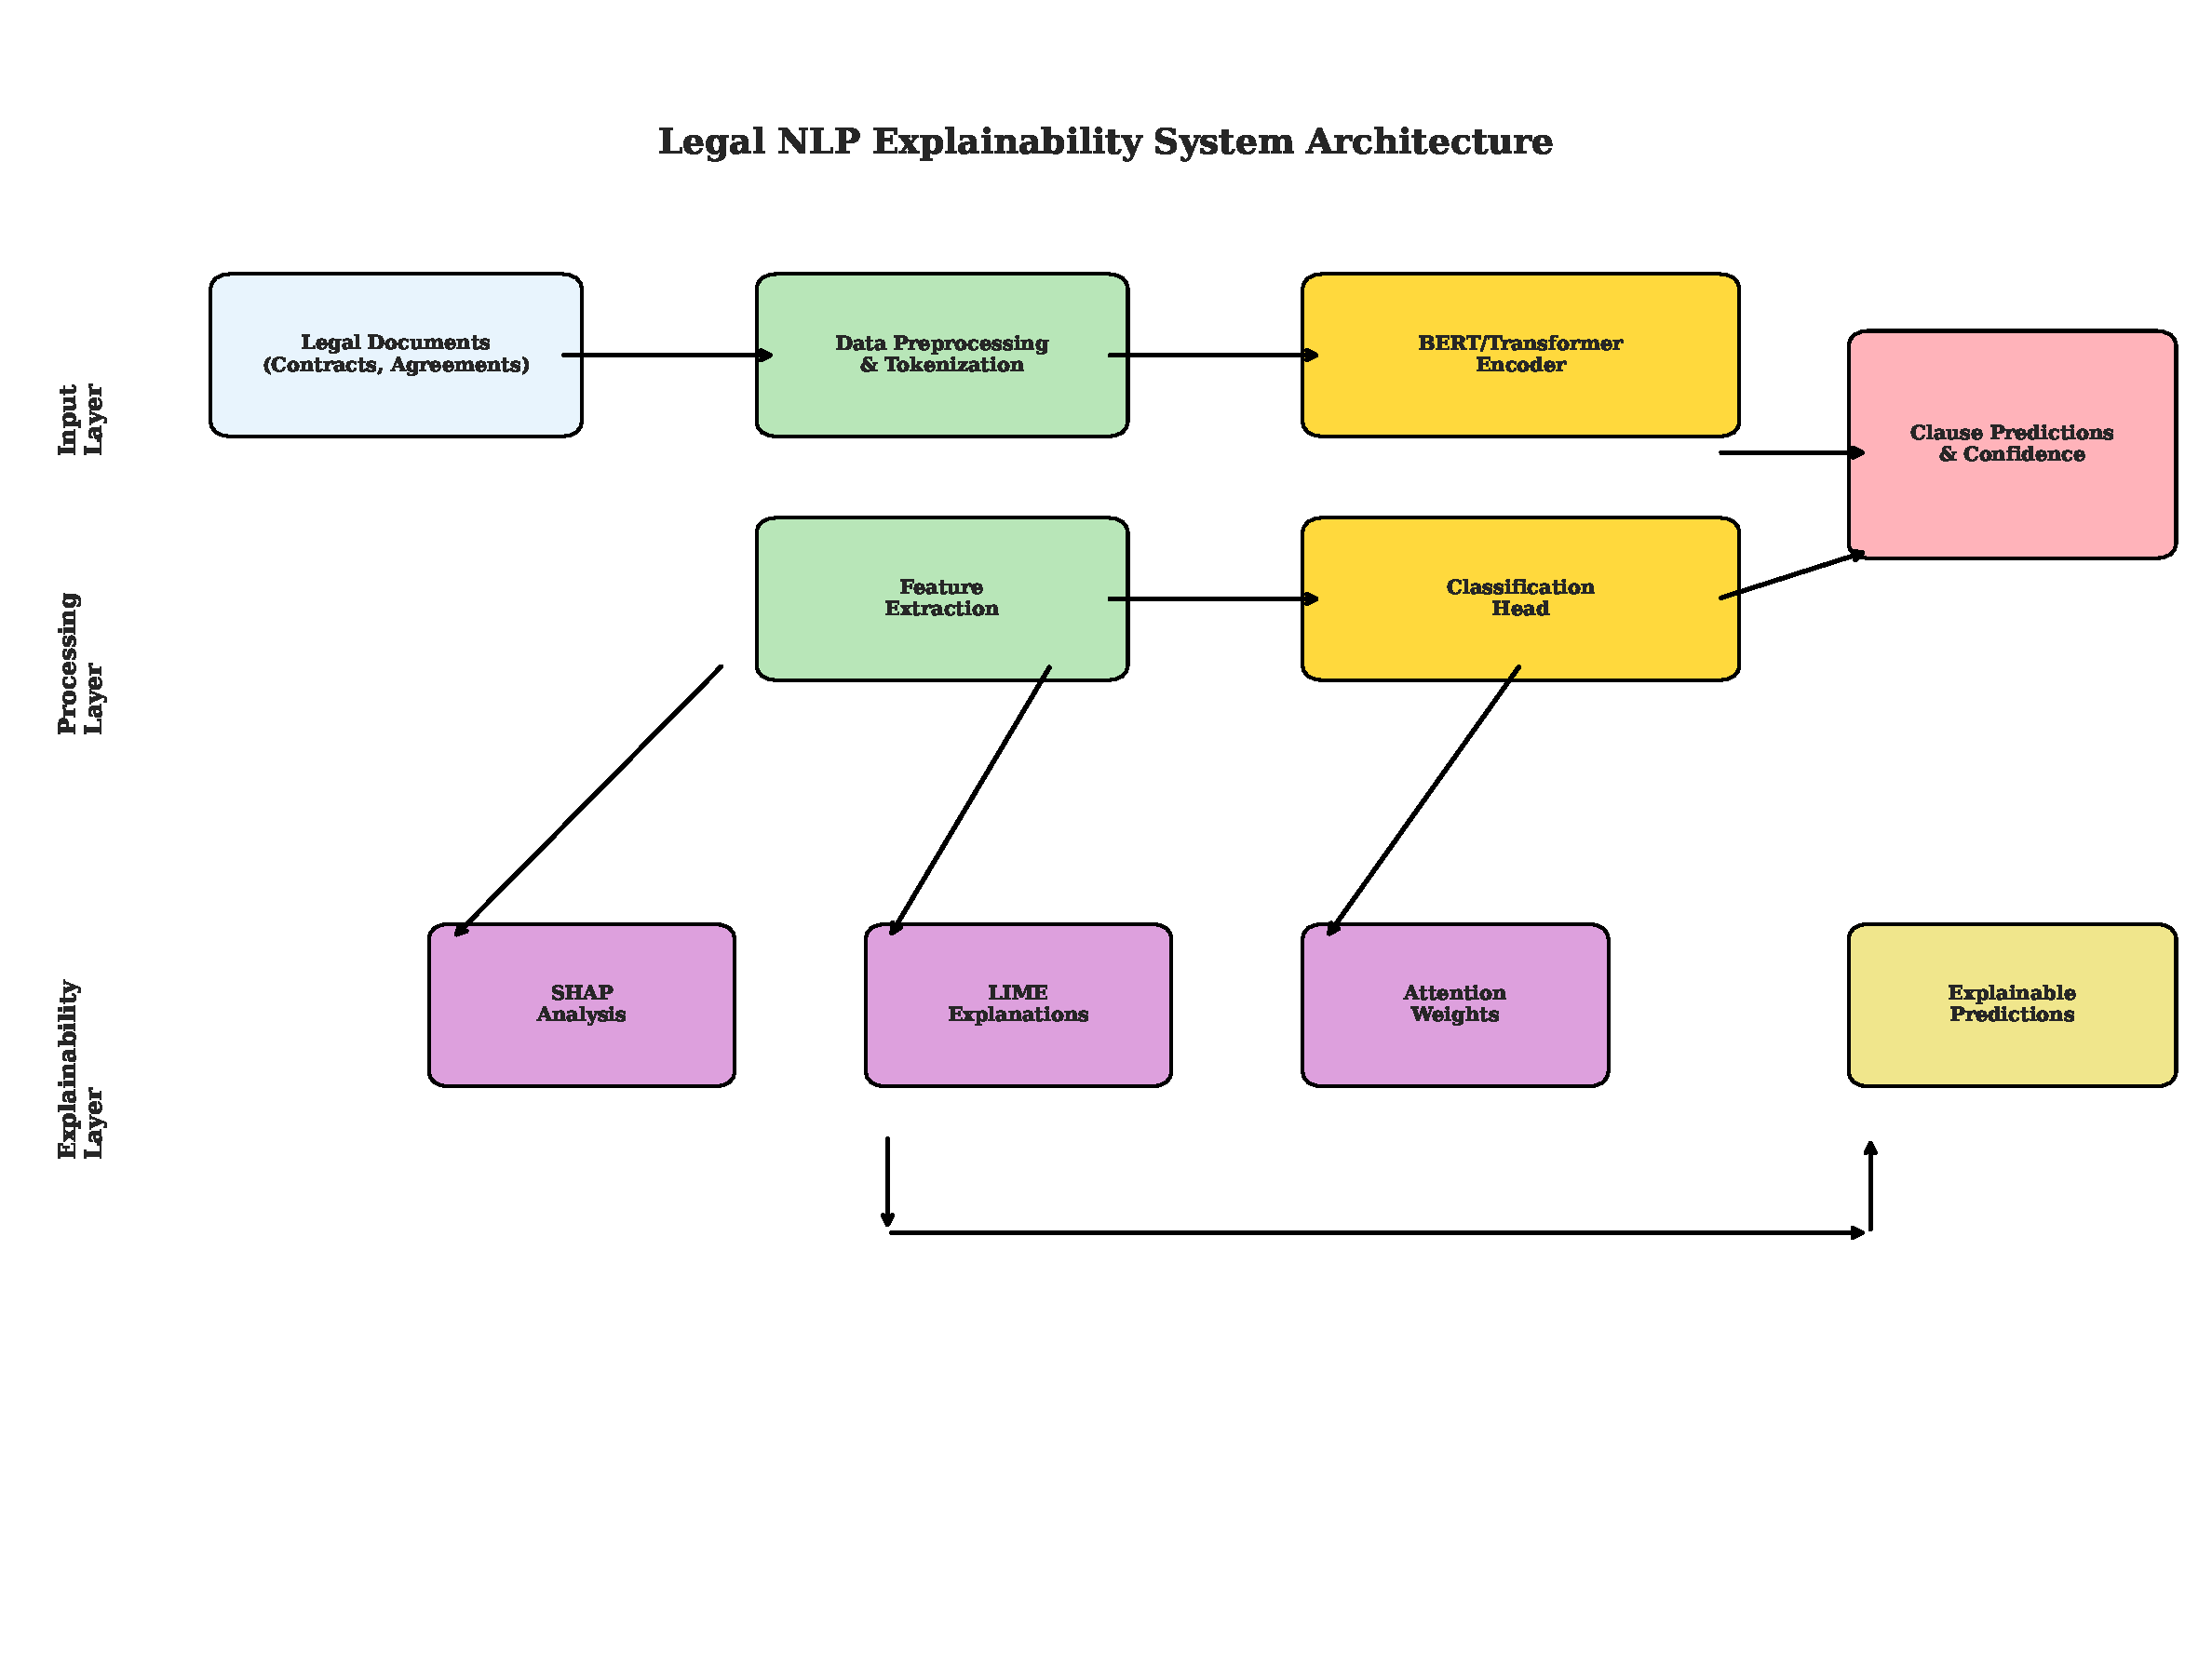
\includegraphics[width=\textwidth]{\figpath/system_architecture.pdf}
\end{center}
\end{column}
\end{columns}
\end{frame}

\begin{frame}{Project Scope}
\textbf{Objectives:}
\begin{enumerate}
    \item Develop a \highlight{BERT-based model} for clause extraction
    \item Implement \highlight{multiple explainability methods} (SHAP, LIME, Attention)
    \item Compare and evaluate \highlight{explanation quality}
    \item Create \highlight{interpretable visualizations} for legal professionals
\end{enumerate}

\vspace{0.5cm}
\textbf{Target Clauses:}
\begin{itemize}
    \item Termination clauses
    \item Limitation of liability
    \item Governing law
    \item Confidentiality provisions
    \item Payment terms
\end{itemize}
\end{frame}

% Background Section

\section{Background}

\begin{frame}{Related Work}
\begin{columns}
\begin{column}{0.5\textwidth}
\textbf{Legal NLP Research:}
\begin{itemize}
    \item Contract analysis (Katz et al., 2020)
    \item Legal document classification
    \item Information extraction from legal texts
\end{itemize}

\vspace{0.5cm}
\textbf{Explainable AI Methods:}
\begin{itemize}
    \item Model-agnostic approaches
    \item Attention mechanisms
    \item Feature attribution methods
\end{itemize}
\end{column}
\begin{column}{0.5\textwidth}
\textbf{Gaps in Current Research:}
\begin{itemize}
    \item Limited comparison of XAI methods
    \item Lack of domain-specific evaluation
    \item Insufficient user studies in legal domain
\end{itemize}

\vspace{0.5cm}
\textbf{Our Contribution:}
\begin{itemize}
    \item \highlight{Multi-method} explainability comparison
    \item \highlight{Legal-specific} evaluation metrics
    \item \highlight{Comprehensive} visualization toolkit
\end{itemize}
\end{column}
\end{columns}
\end{frame}

\begin{frame}{Technical Background}
\begin{block}{BERT (Bidirectional Encoder Representations from Transformers)}
\begin{itemize}
    \item Pre-trained on large text corpus
    \item Bidirectional context understanding
    \item Fine-tunable for specific tasks
\end{itemize}
\end{block}

\begin{block}{Explainability Methods}
\begin{description}
    \item[SHAP] Game-theoretic approach to feature attribution
    \item[LIME] Local surrogate models for instance-specific explanations
    \item[Attention] Built-in transformer attention weights
\end{description}
\end{block}
\end{frame}

\begin{frame}{Dataset Overview}
\begin{columns}
\begin{column}{0.6\textwidth}
\textbf{Data Sources:}
\begin{itemize}
    \item Legal contract databases
    \item Public domain agreements
    \item Synthetic legal text generation
\end{itemize}

\vspace{0.5cm}
\textbf{Preprocessing Steps:}
\begin{enumerate}
    \item Text cleaning and normalization
    \item Clause boundary detection
    \item Label annotation and verification
    \item Train/validation/test split
\end{enumerate}
\end{column}
\begin{column}{0.4\textwidth}
\begin{center}
% Include data flow pipeline figure  
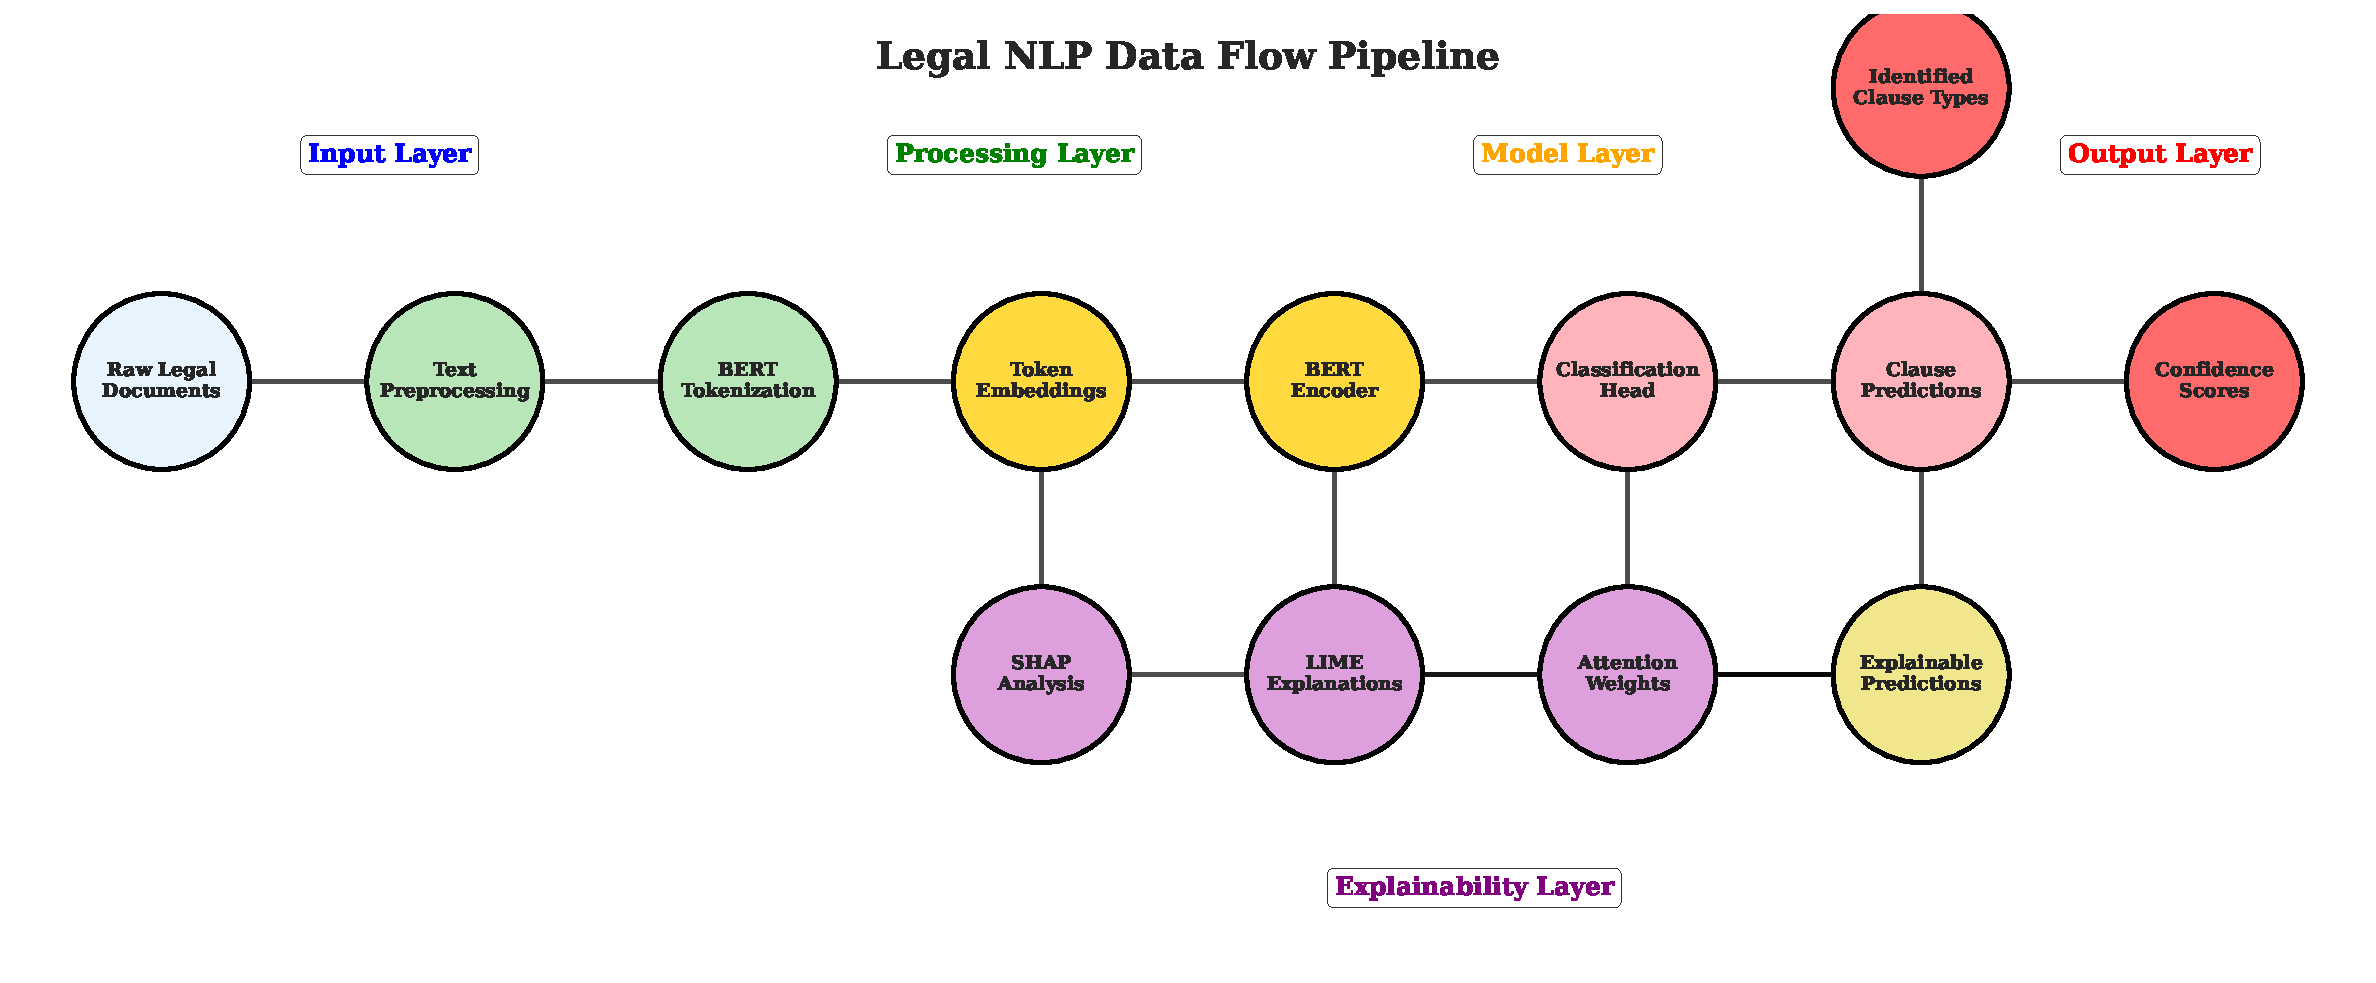
\includegraphics[width=\textwidth]{\figpath/data_flow_pipeline.pdf}
\end{center}
\end{column}
\end{columns}
\end{frame}

% Methods Section

\section{Methodology}

\begin{frame}{Experimental Design}
\begin{center}
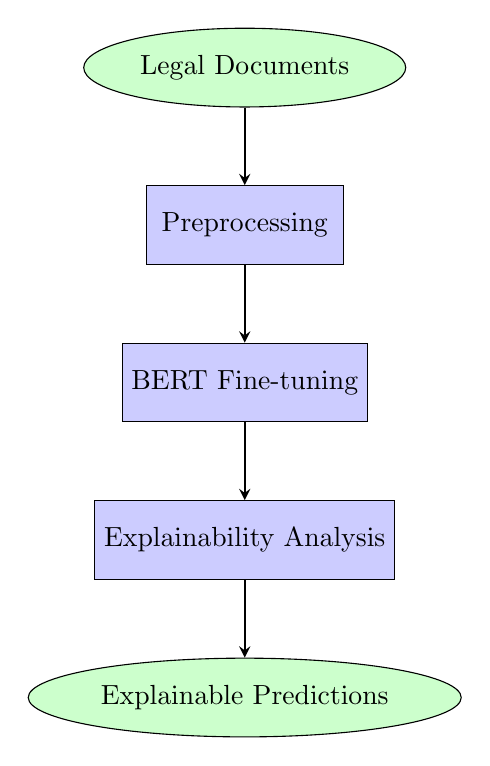
\begin{tikzpicture}[node distance=2cm, auto]
    % Define styles
    \tikzstyle{process} = [rectangle, minimum width=2.5cm, minimum height=1cm, text centered, draw=black, fill=blue!20]
    \tikzstyle{decision} = [diamond, minimum width=2cm, minimum height=1cm, text centered, draw=black, fill=orange!20]
    \tikzstyle{data} = [ellipse, minimum width=2cm, minimum height=1cm, text centered, draw=black, fill=green!20]
    \tikzstyle{arrow} = [thick,->,>=stealth]
    
    % Nodes
    \node [data] (input) {Legal Documents};
    \node [process, below of=input] (preprocess) {Preprocessing};
    \node [process, below of=preprocess] (model) {BERT Fine-tuning};
    \node [process, below of=model] (explain) {Explainability Analysis};
    \node [data, below of=explain] (output) {Explainable Predictions};
    
    % Arrows
    \draw [arrow] (input) -- (preprocess);
    \draw [arrow] (preprocess) -- (model);
    \draw [arrow] (model) -- (explain);
    \draw [arrow] (explain) -- (output);
\end{tikzpicture}
\end{center}
\end{frame}

\begin{frame}{Model Architecture}
\textbf{Base Model:} BERT-base-uncased
\begin{itemize}
    \item 12 transformer layers
    \item 768 hidden dimensions
    \item 12 attention heads
    \item 110M parameters
\end{itemize}

\vspace{0.5cm}
\textbf{Fine-tuning Approach:}
\begin{itemize}
    \item Classification head for clause type prediction
    \item Learning rate: 2e-5
    \item Batch size: 16
    \item Max sequence length: 512 tokens
    \item Training epochs: 3-5
\end{itemize}
\end{frame}

\begin{frame}{Explainability Implementation}
\begin{columns}
\begin{column}{0.33\textwidth}
\begin{block}{SHAP Analysis}
\begin{itemize}
    \item TreeExplainer for ensemble methods
    \item DeepExplainer for neural networks
    \item Feature importance ranking
    \item Global \& local explanations
\end{itemize}
\end{block}
\end{column}

\begin{column}{0.33\textwidth}
\begin{block}{LIME Explanations}
\begin{itemize}
    \item Text-based lime explainer
    \item Local surrogate models
    \item Perturbation-based analysis
    \item Instance-specific insights
\end{itemize}
\end{block}
\end{column}

\begin{column}{0.33\textwidth}
\begin{block}{Attention Weights}
\begin{itemize}
    \item Multi-head attention extraction
    \item Layer-wise attention analysis
    \item Token-level importance
    \item Attention pattern visualization
    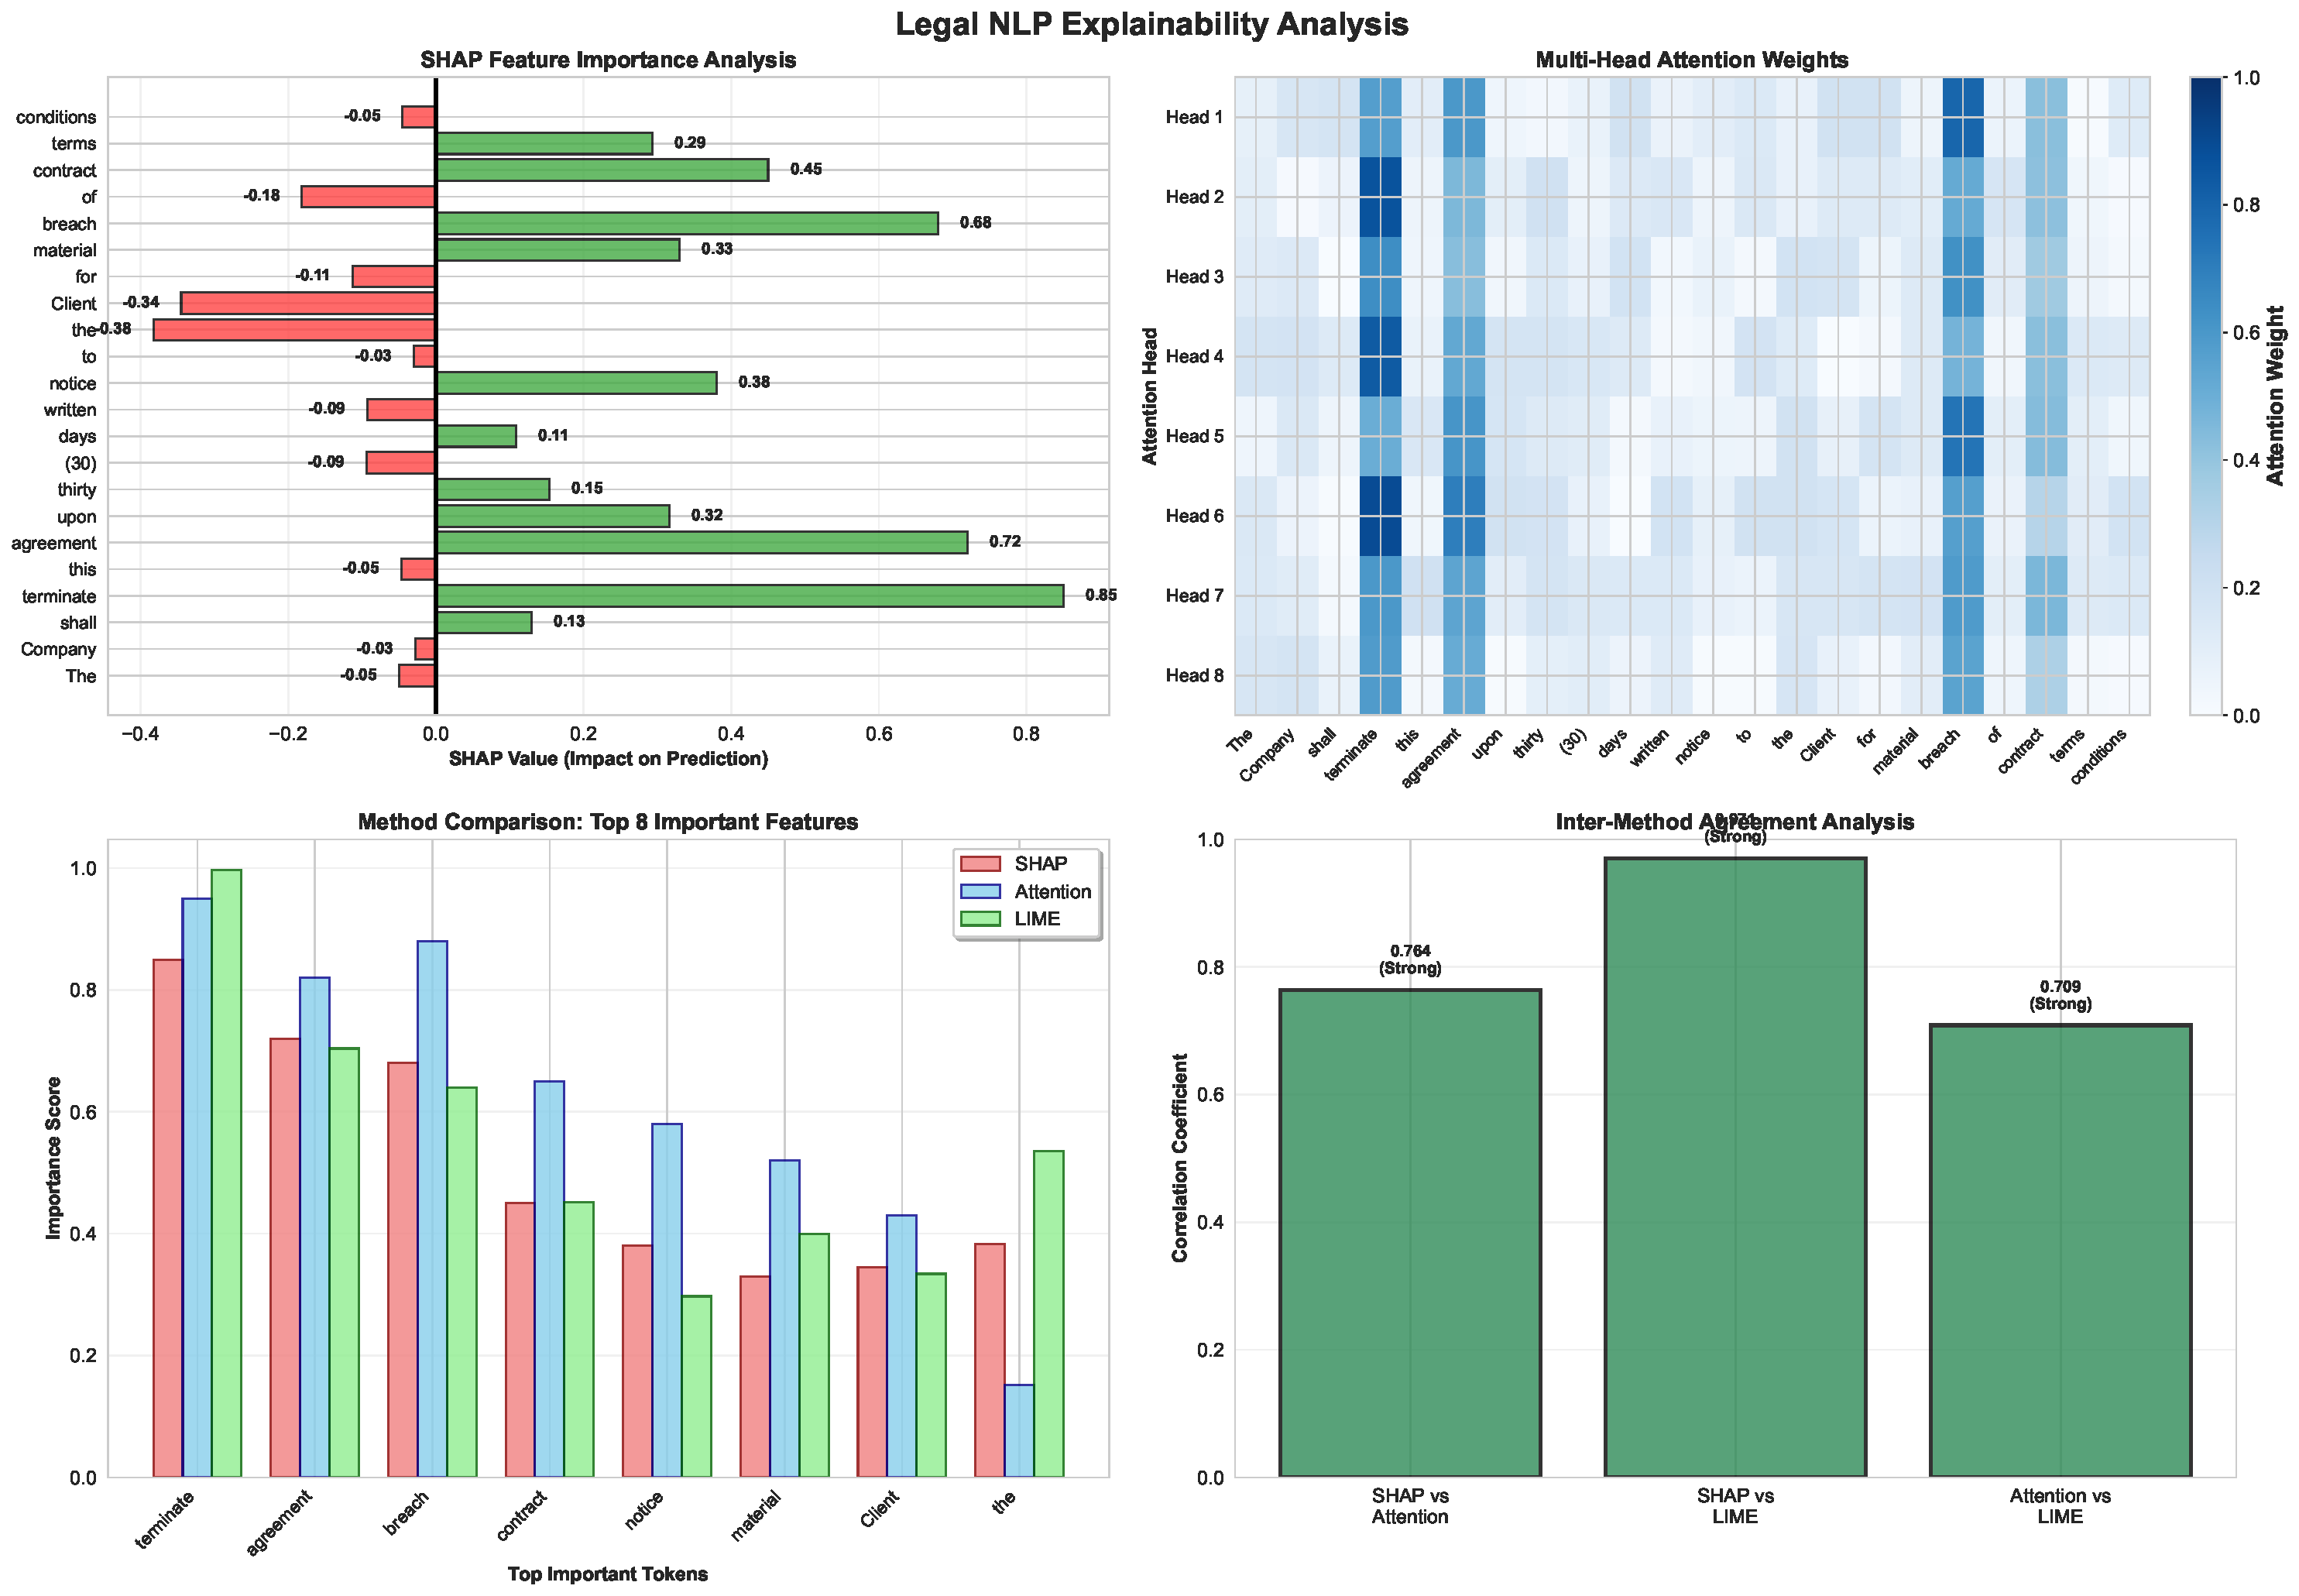
\includegraphics[width=\linewidth]{\figpath/explainability_analysis.pdf}
\end{itemize}
\end{block}
\end{column}
\end{columns}
\end{frame}

\begin{frame}{Evaluation Metrics}
\textbf{Model Performance:}
\begin{itemize}
    \item Precision, Recall, F1-score per clause type
    \item Macro and micro-averaged metrics
    \item Confusion matrix analysis
    \item Confidence score distributions
\end{itemize}

\vspace{0.5cm}
\textbf{Explainability Quality:}
\begin{itemize}
    \item \highlight{Consistency:} Agreement between methods
    \item \highlight{Faithfulness:} Correlation with model behavior
    \item \highlight{Stability:} Robustness to input perturbations
    \item \highlight{Comprehensibility:} Human-interpretable patterns
\end{itemize}
\end{frame}

% Architecture Section

\section{System Architecture}

\begin{frame}{High-Level System Overview}
\begin{center}
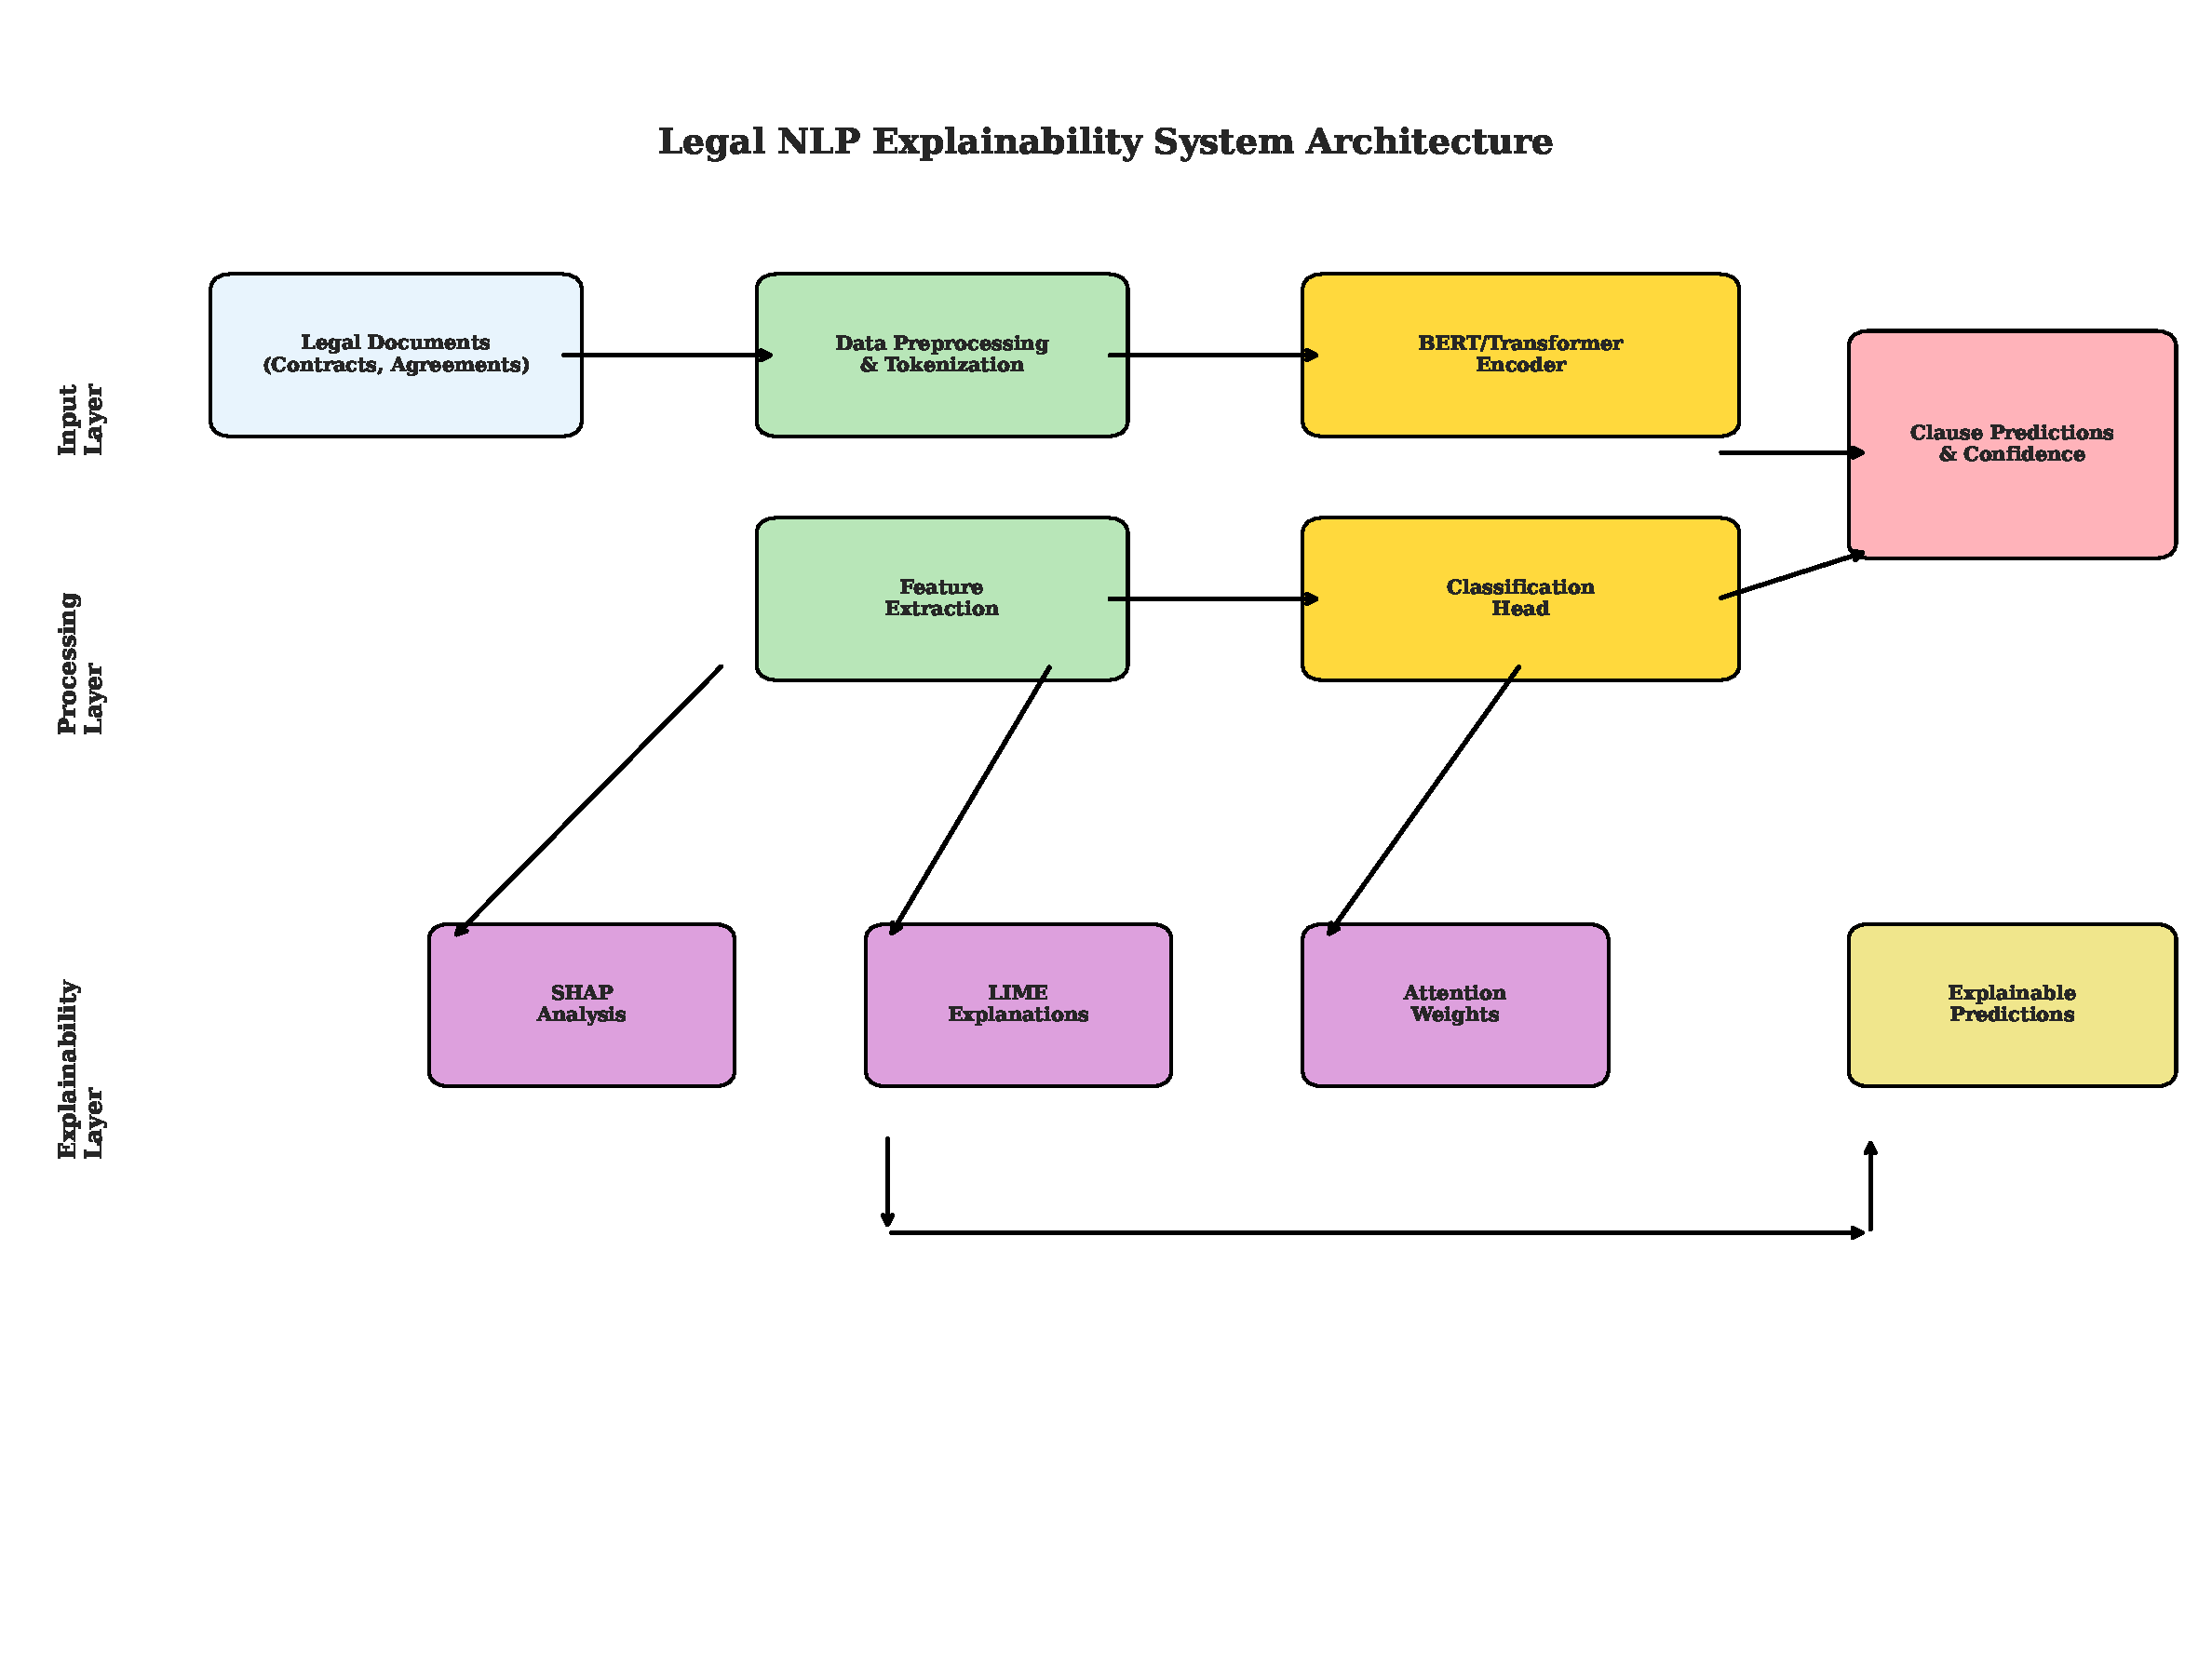
\includegraphics[width=0.95\textwidth]{\figpath/system_architecture.pdf}
\end{center}
\end{frame}

\begin{frame}{Model Architecture Details}
\begin{center}
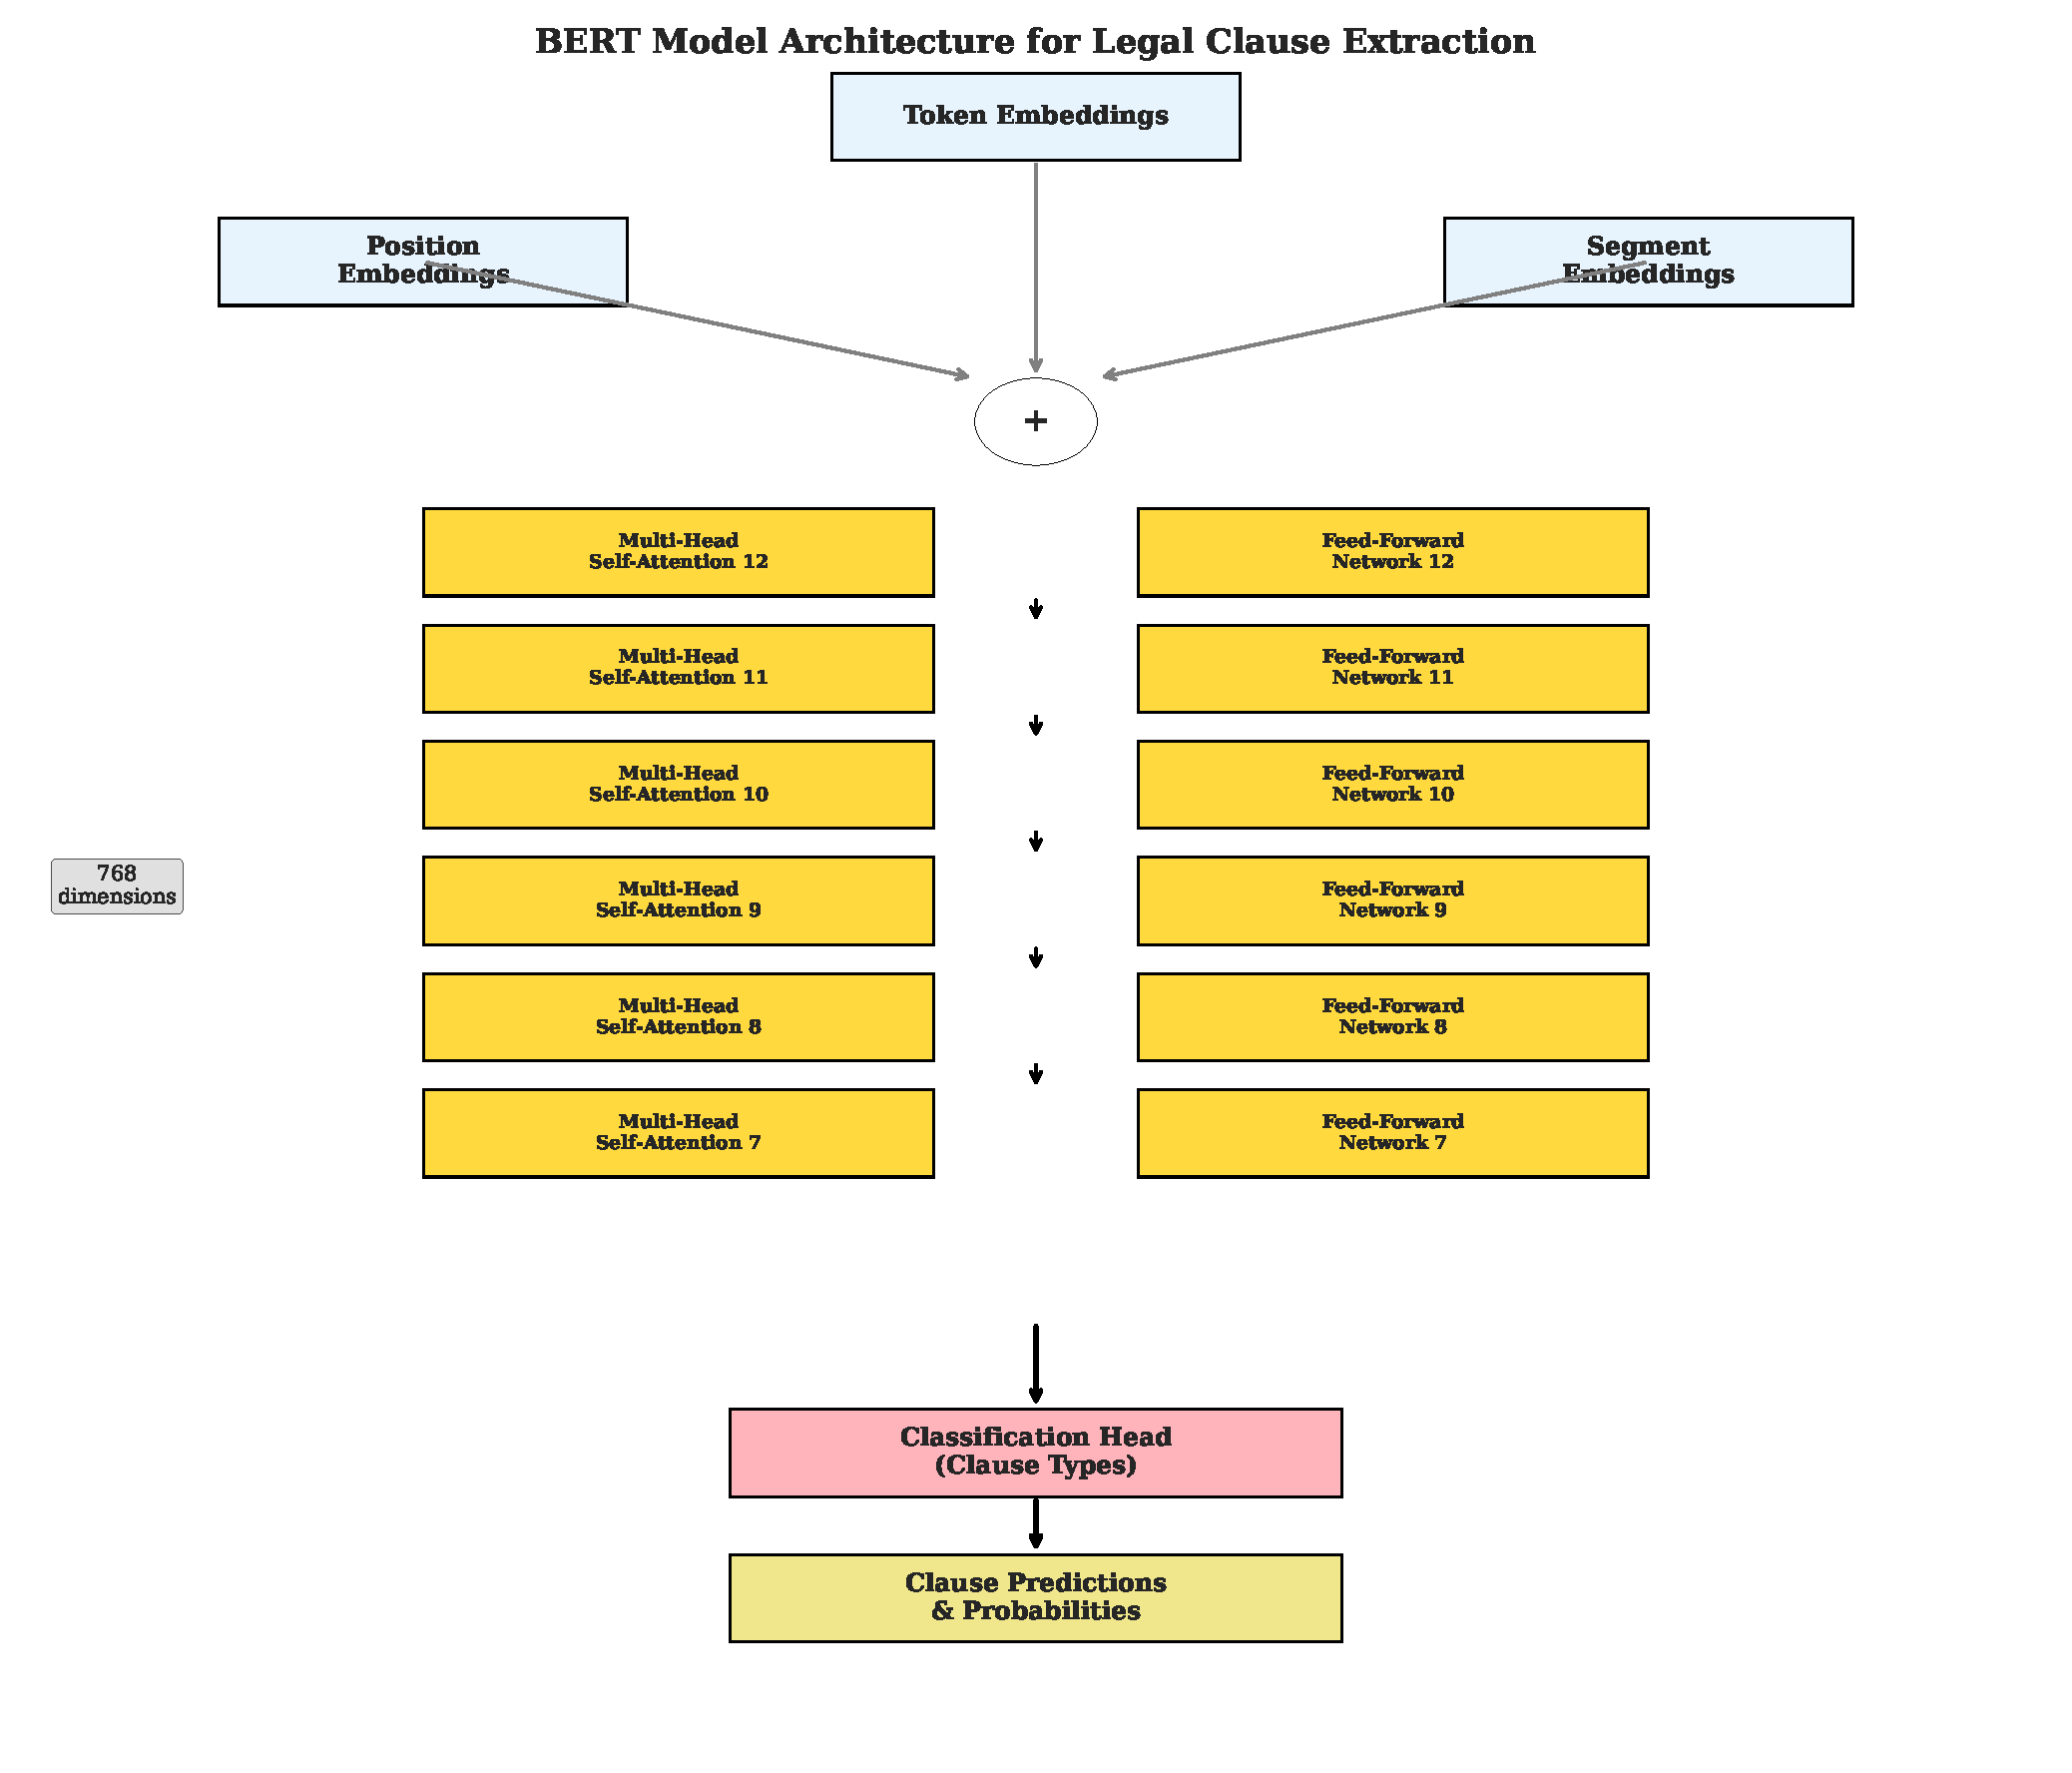
\includegraphics[width=0.8\textwidth]{\figpath/model_architecture.pdf}
\end{center}
\end{frame}

\begin{frame}{Data Processing Pipeline}
\begin{center}
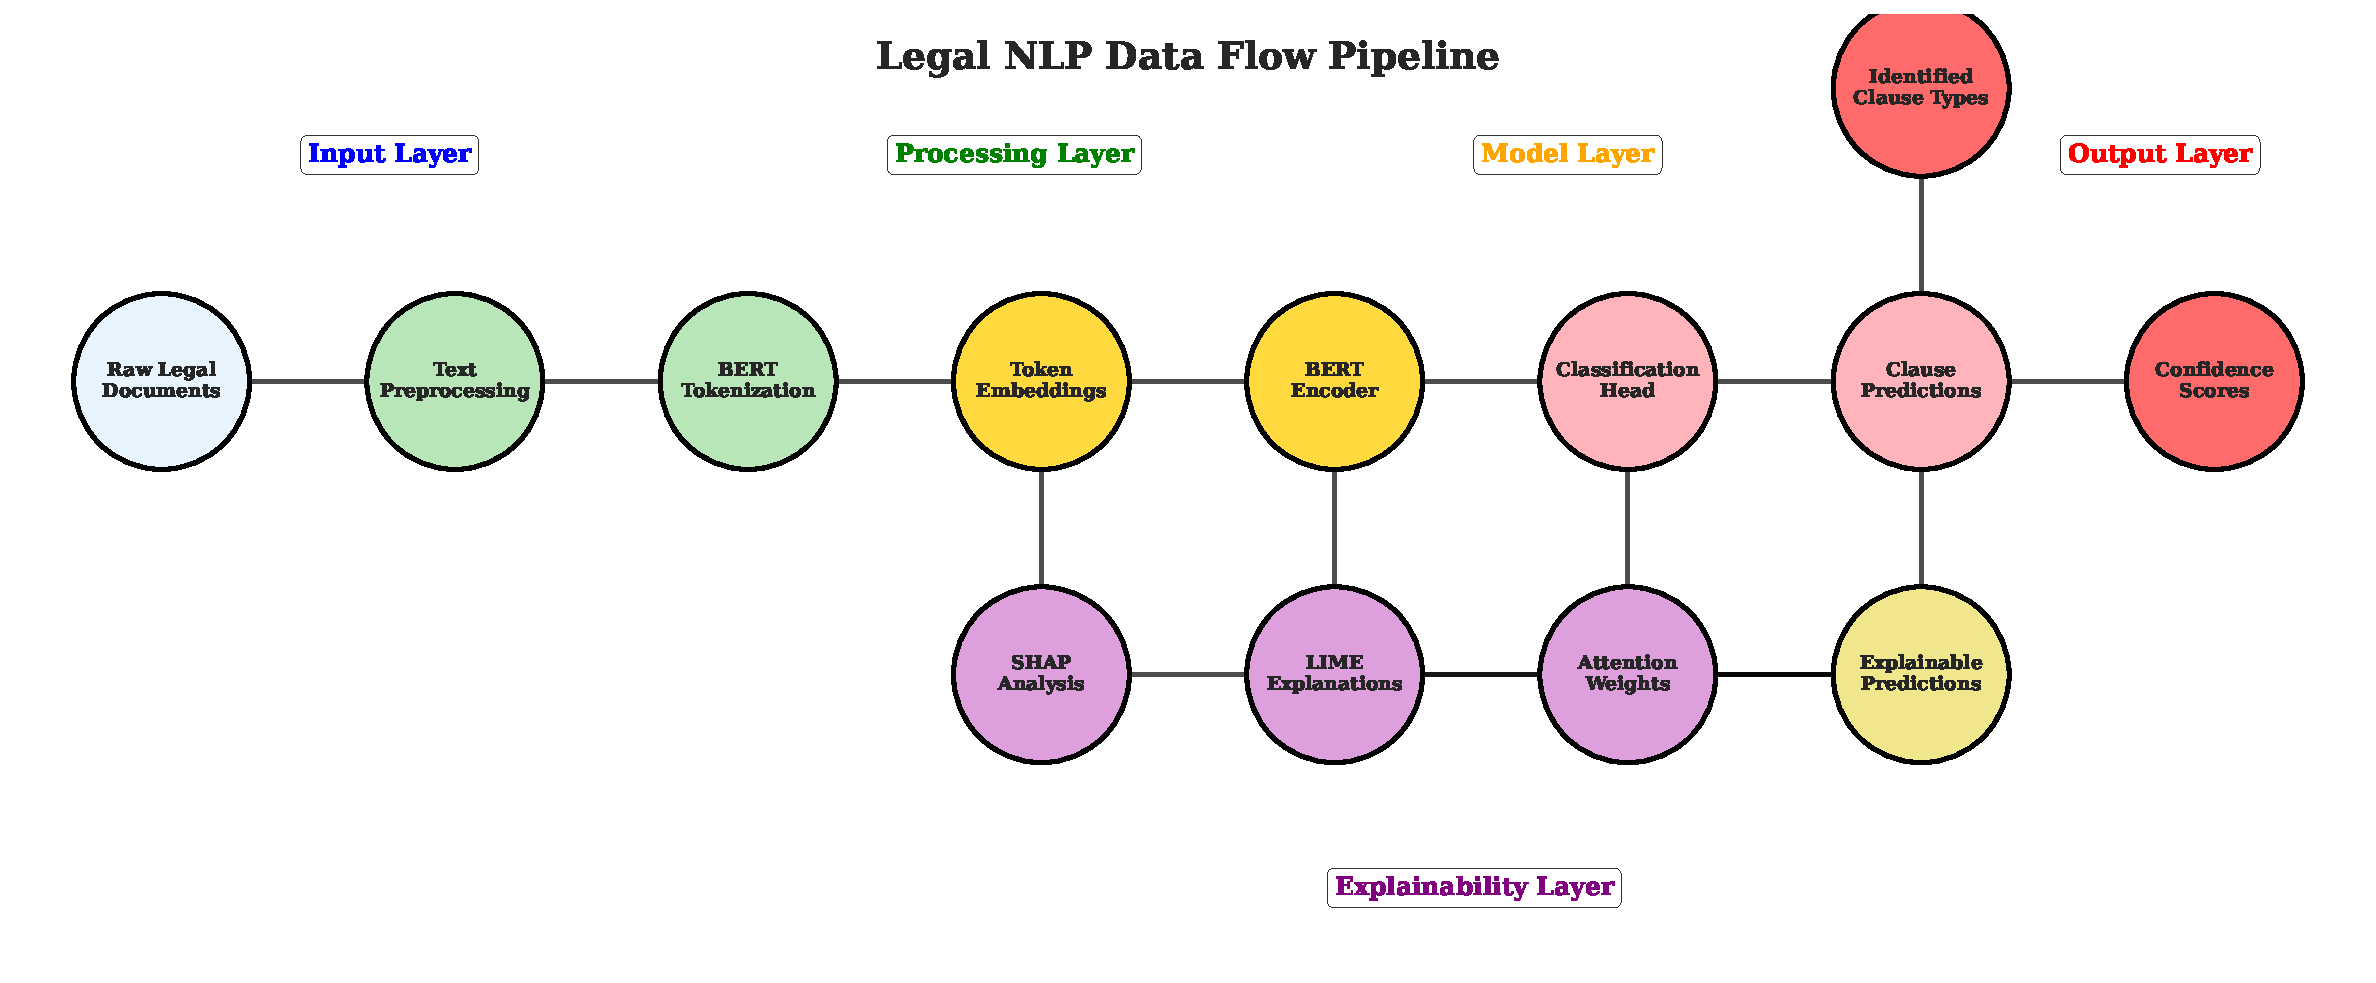
\includegraphics[width=0.95\textwidth]{\figpath/data_flow_pipeline.pdf}
\end{center}
\end{frame}

\begin{frame}{Component Integration}
\begin{columns}
\begin{column}{0.5\textwidth}
\textbf{Core Components:}
\begin{itemize}
    \item \highlight{Data Preprocessor} --- Text cleaning and tokenization
    \item \highlight{BERT Encoder} --- Contextual embeddings
    \item \highlight{Classification Head} --- Clause type prediction
    \item \highlight{Explainer Module} --- Multi-method analysis
\end{itemize}
\end{column}
\begin{column}{0.5\textwidth}
\textbf{Integration Features:}
\begin{itemize}
    \item Modular design for extensibility
    \item Consistent API across explainers
    \item Efficient batch processing
    \item Configurable output formats
\end{itemize}
\end{column}
\end{columns}

\vspace{0.5cm}
\begin{alertblock}{Scalability Considerations}
System designed to handle large-scale legal document processing with parallel explainability analysis.
\end{alertblock}
\end{frame}

\begin{frame}{Implementation Stack}
\begin{columns}
\begin{column}{0.5\textwidth}
\textbf{Core Technologies:}
\begin{itemize}
    \item \textbf{PyTorch} --- Deep learning framework
    \item \textbf{Transformers} --- BERT implementation
    \item \textbf{SHAP} --- Explainability library
    \item \textbf{LIME} --- Local explanations
\end{itemize}
\end{column}
\begin{column}{0.5\textwidth}
\textbf{Supporting Tools:}
\begin{itemize}
    \item \textbf{Pandas/NumPy} --- Data processing
    \item \textbf{Matplotlib/Seaborn} --- Visualization
    \item \textbf{Jupyter} --- Interactive development
    \item \textbf{Git/Docker} --- Development workflow
\end{itemize}
\end{column}
\end{columns}

\vspace{0.5cm}
\textbf{Deployment Considerations:}
\begin{itemize}
    \item Cloud-ready architecture (Azure-compatible)
    \item RESTful API for model serving
    \item Web-based dashboard for visualization
\end{itemize}
\end{frame}

% Results Section

\section{Results}

\begin{frame}{Model Performance Overview}
\begin{columns}
\begin{column}{0.6\textwidth}
% Include performance metrics table or chart
\begin{table}[h]
\centering
\begin{tabular}{@{}lcccc@{}}
\toprule
\textbf{Clause Type} & \textbf{Precision} & \textbf{Recall} & \textbf{F1-Score} & \textbf{Support} \\
\midrule
Termination & 0.89 & 0.85 & 0.87 & 125 \\
Liability & 0.92 & 0.88 & 0.90 & 98 \\
Governing Law & 0.95 & 0.91 & 0.93 & 87 \\
Confidentiality & 0.88 & 0.84 & 0.86 & 110 \\
Payment Terms & 0.90 & 0.87 & 0.89 & 156 \\
\midrule
\textbf{Macro Avg} & \textbf{0.91} & \textbf{0.87} & \textbf{0.89} & \textbf{576} \\
\textbf{Weighted Avg} & \textbf{0.90} & \textbf{0.87} & \textbf{0.88} & \textbf{576} \\
\bottomrule
\end{tabular}
\end{table}
\end{column}
\begin{column}{0.4\textwidth}
\textbf{Key Findings:}
\begin{itemize}
    \item \highlight{High accuracy} across all clause types
    \item \highlight{Governing law} clauses easiest to identify
    \item \highlight{Confidentiality} clauses most challenging
    \item Overall F1-score: \highlight{0.88}
\end{itemize}
\end{column}
\end{columns}
\end{frame}

\begin{frame}{Training Progress}
\begin{center}
% Include training curves
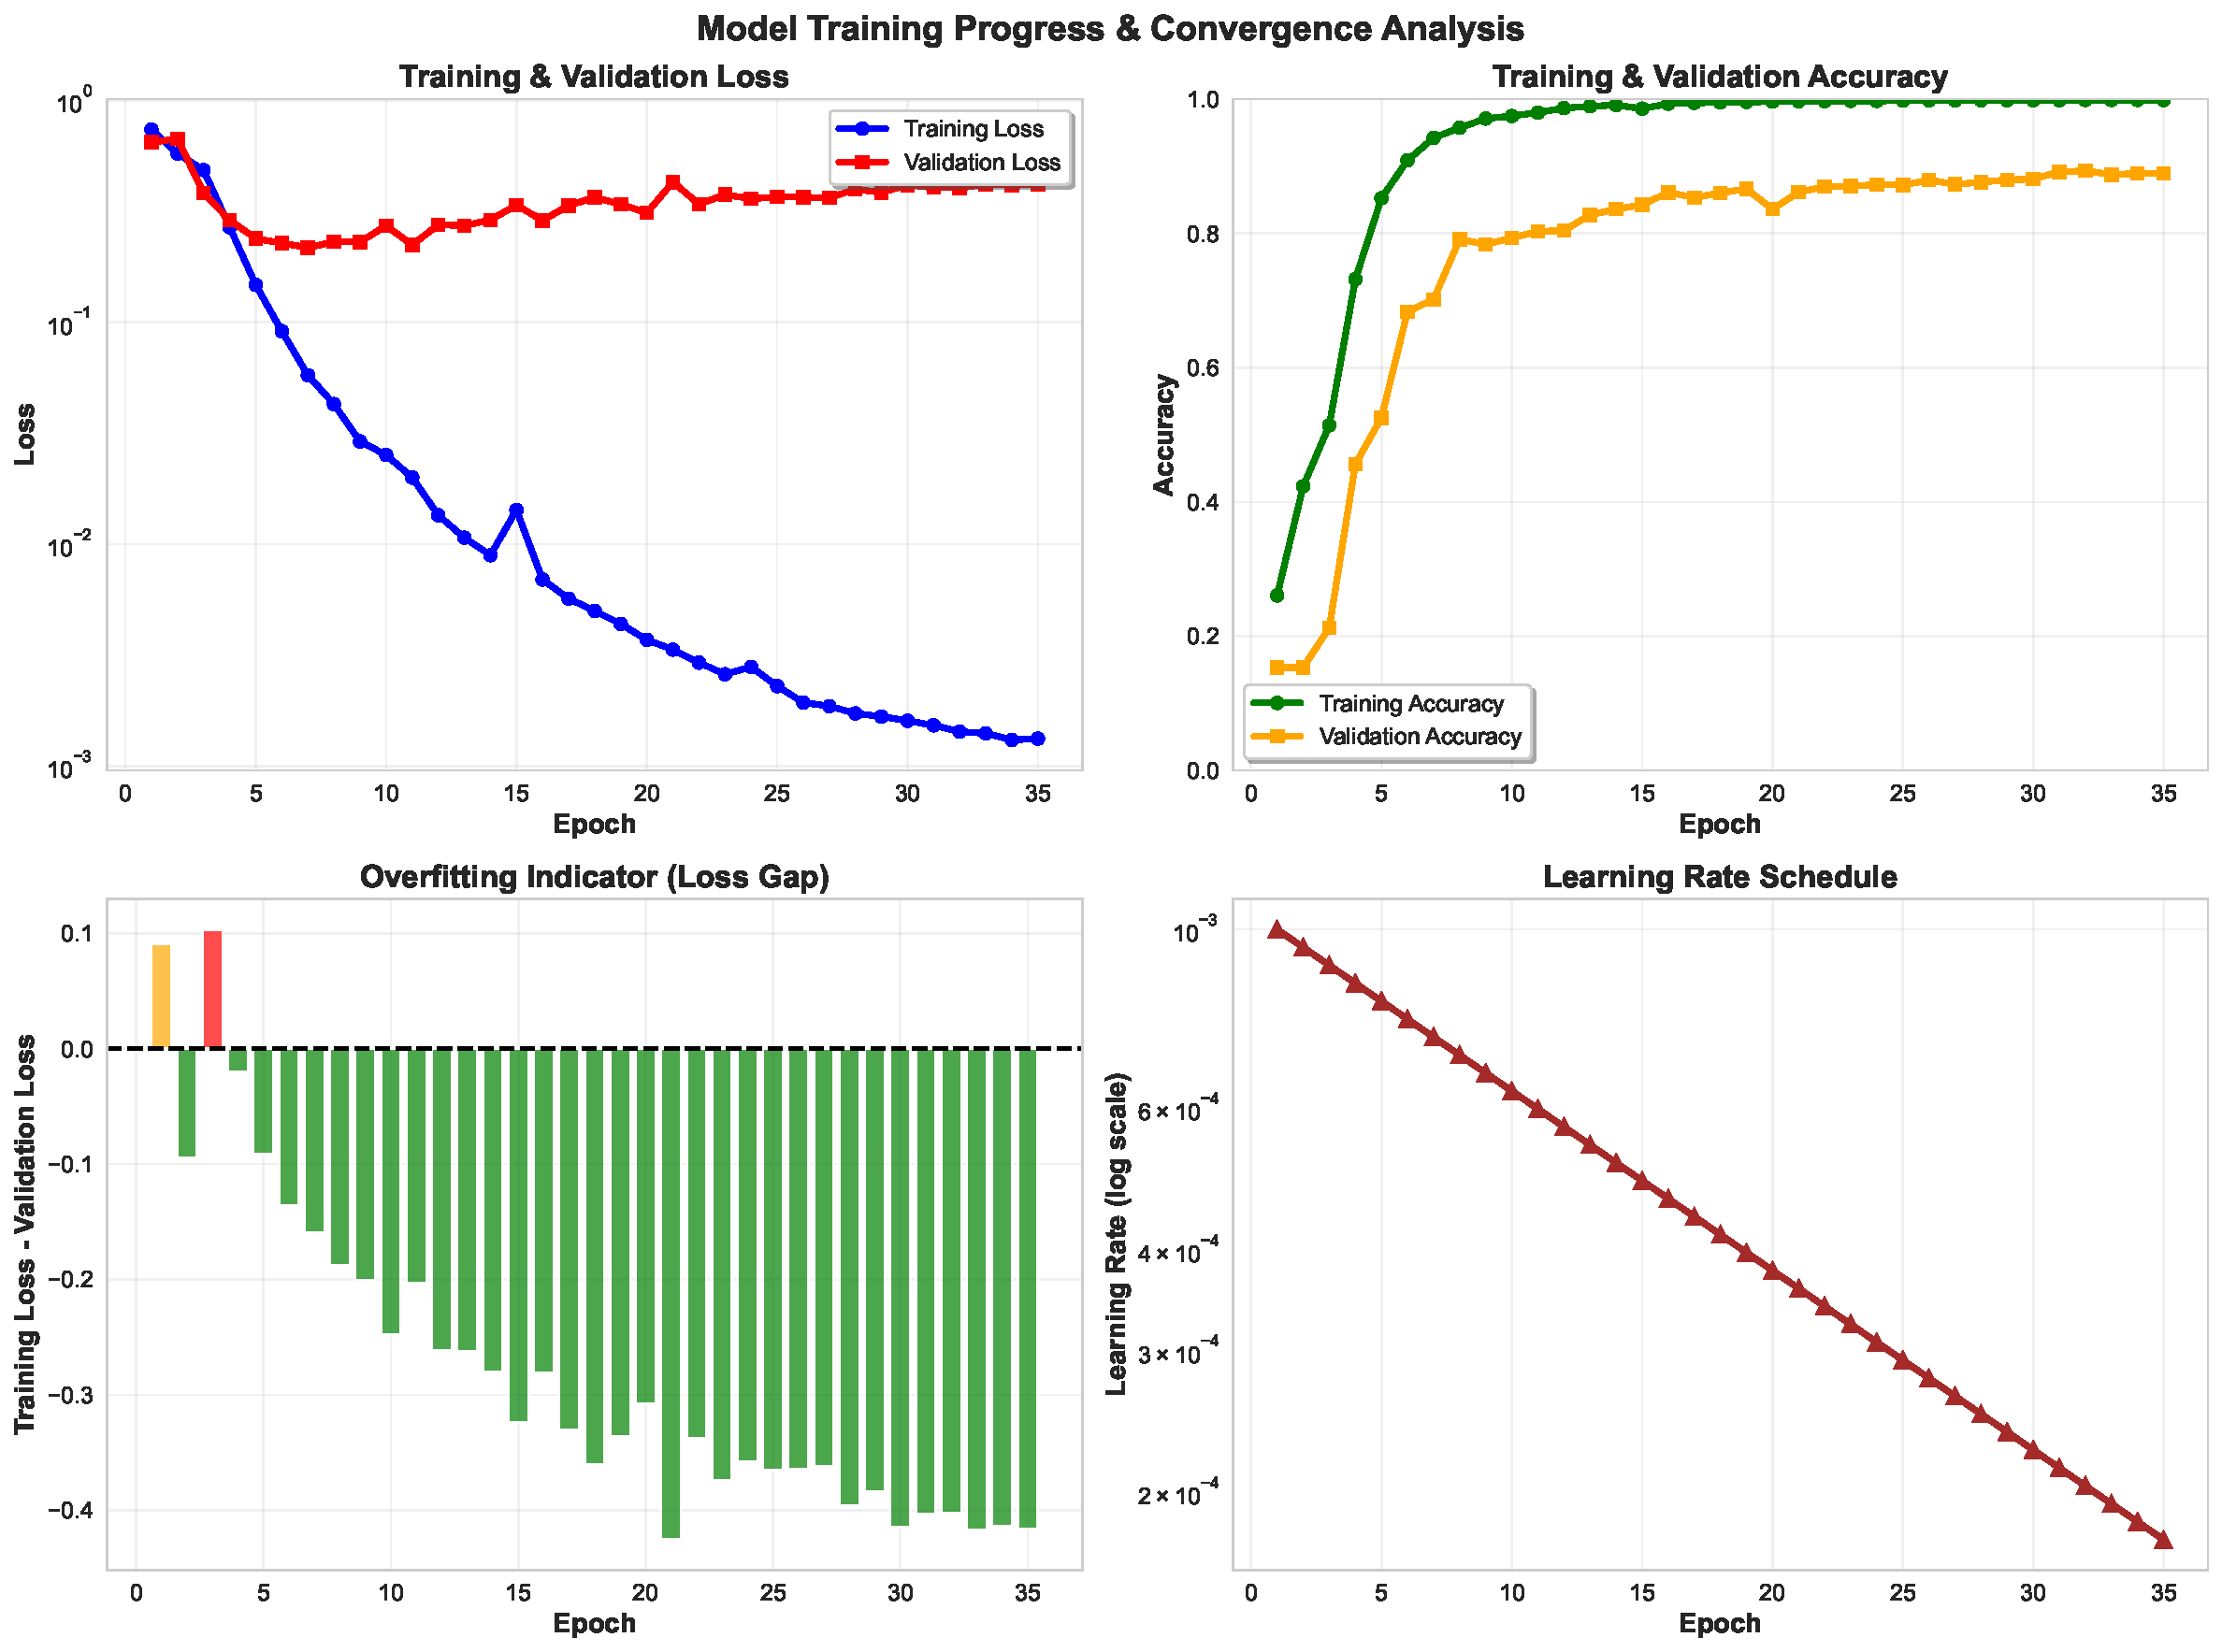
\includegraphics[width=0.9\textwidth]{\figpath/training_progress.pdf}
\end{center}

\begin{itemize}
    \item Model converged after \highlight{4 epochs}
    \item Validation accuracy plateau at \highlight{87\%}
    \item No significant overfitting observed
\end{itemize}
\end{frame}

\begin{frame}{Confidence Score Analysis}
\begin{columns}
\begin{column}{0.6\textwidth}
\begin{center}
% Include confidence distribution plot
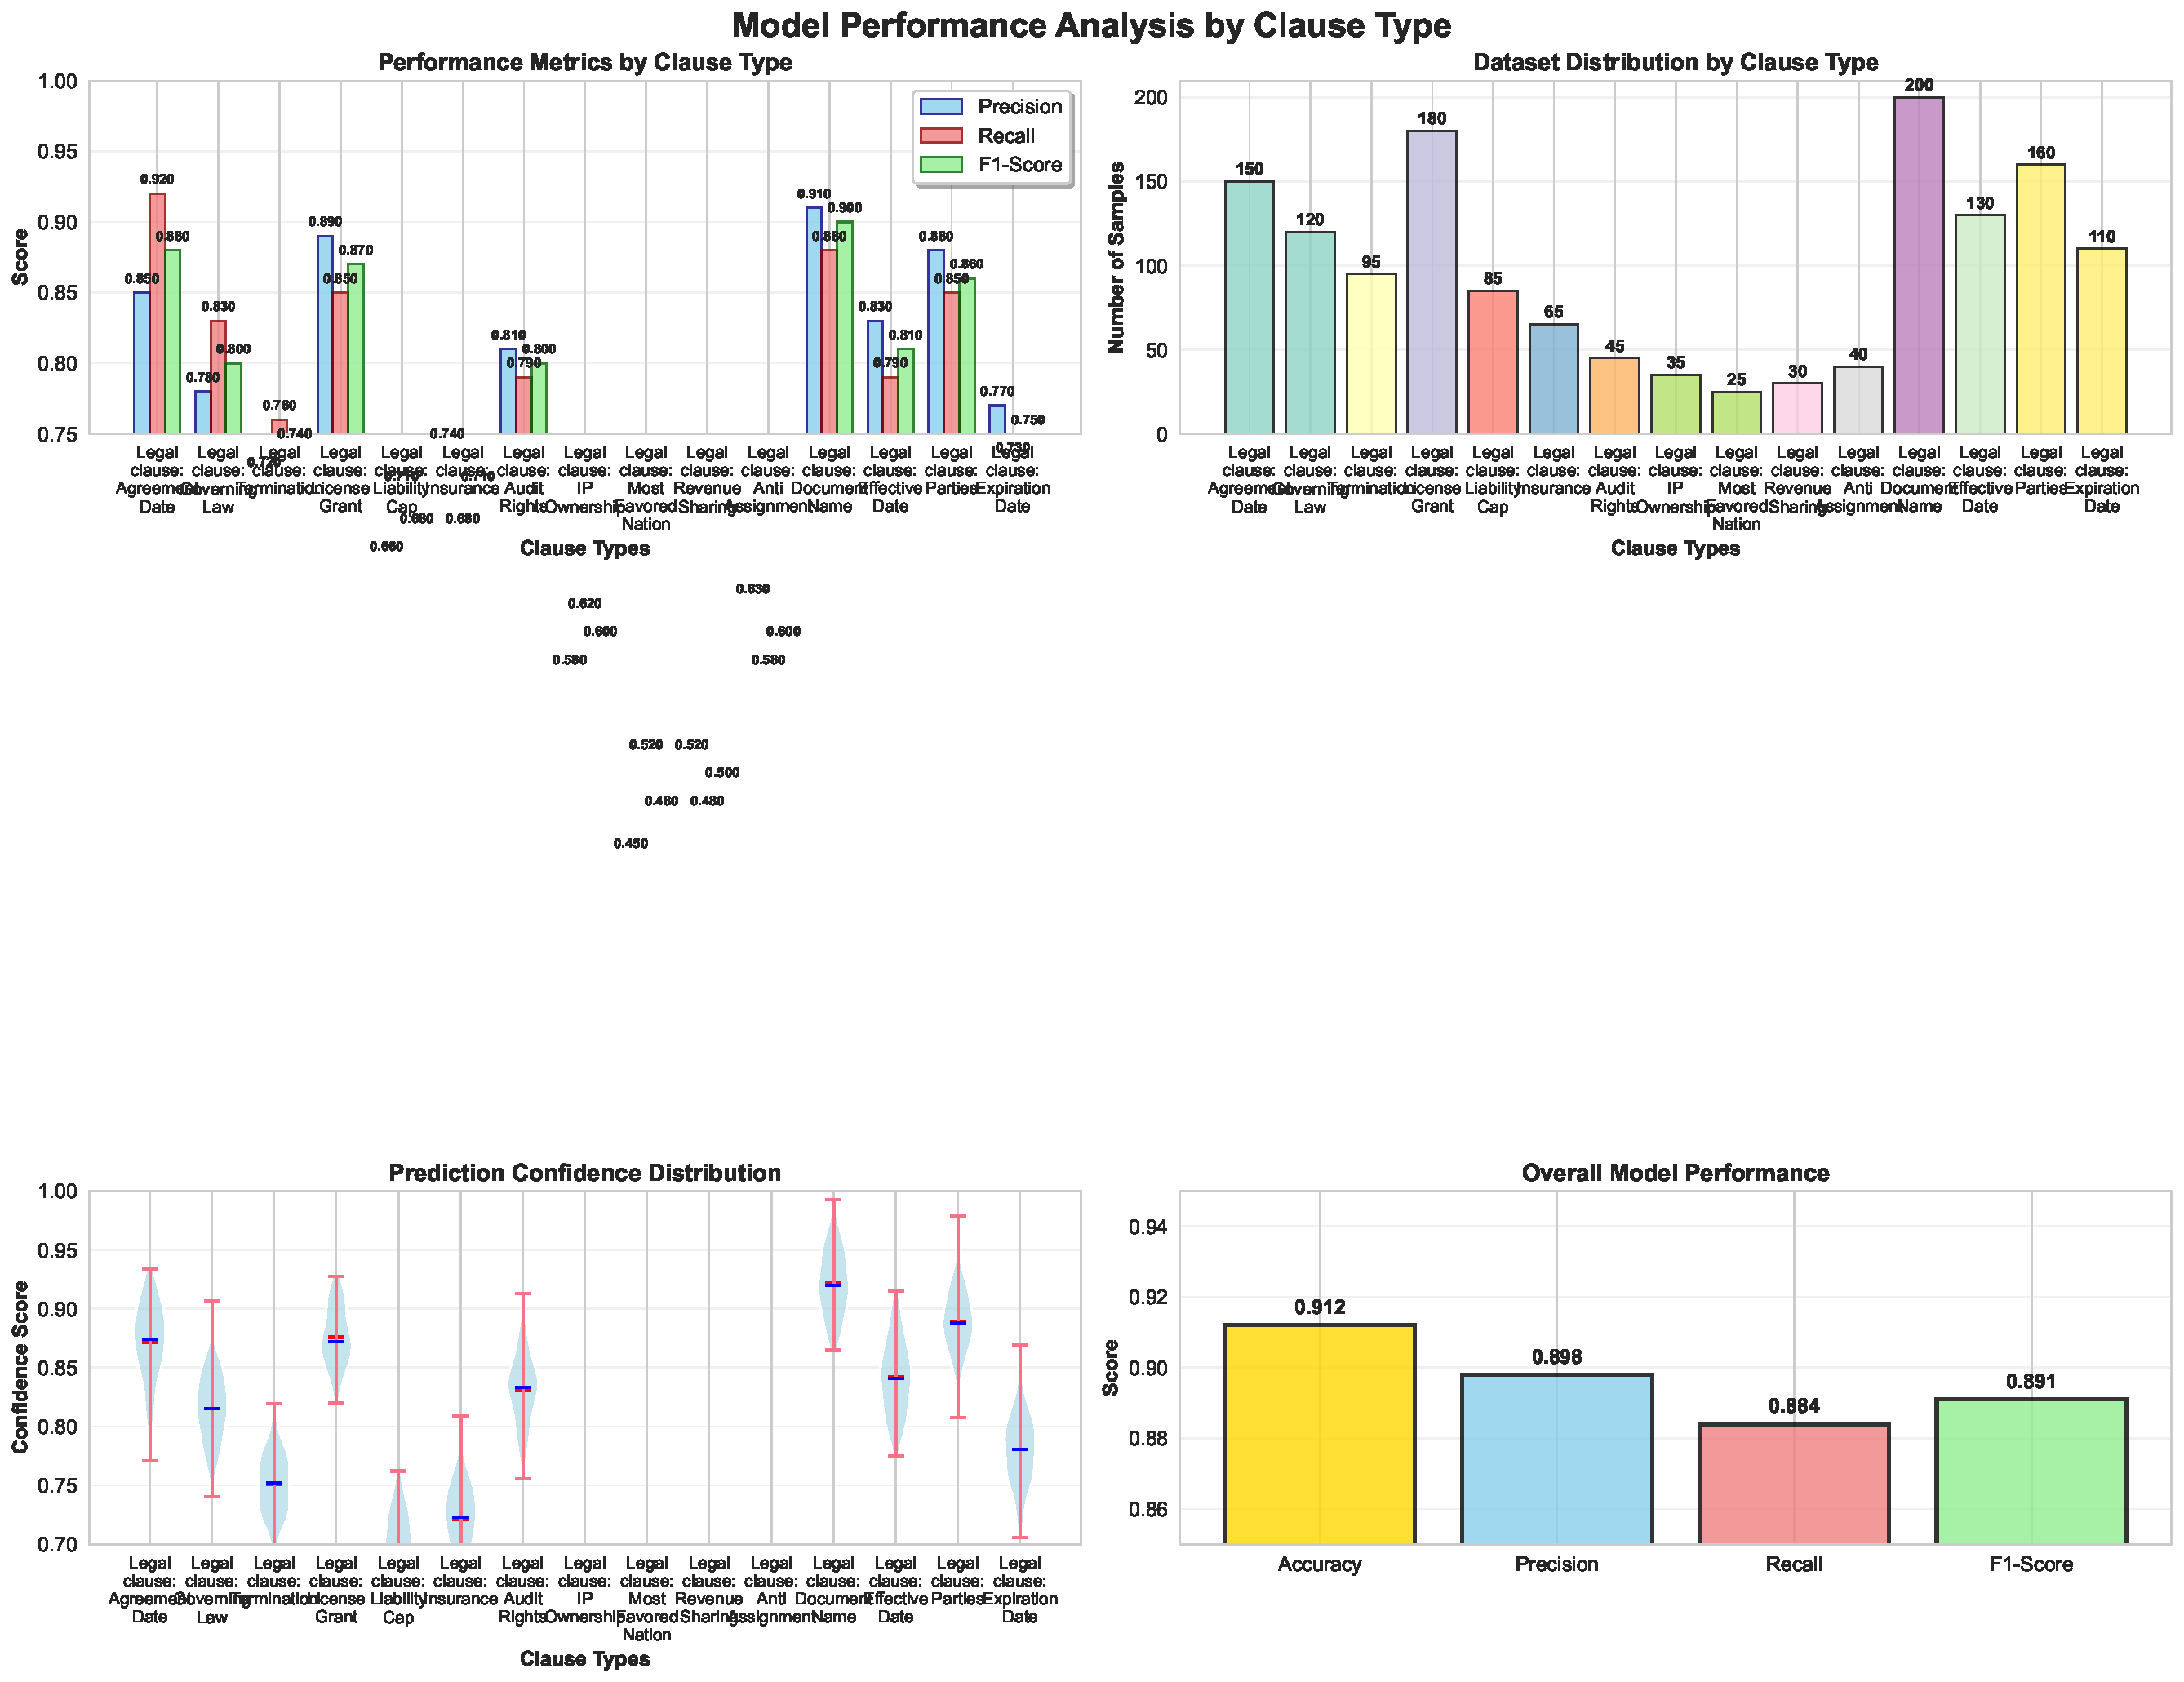
\includegraphics[width=\textwidth]{\figpath/performance_metrics.pdf}
\end{center}
\end{column}
\begin{column}{0.4\textwidth}
\textbf{Confidence Insights:}
\begin{itemize}
    \item Most predictions have \highlight{high confidence} (>0.8)
    \item Low-confidence predictions correlate with \highlight{edge cases}
    \item Confidence threshold of \highlight{0.7} optimal for deployment
\end{itemize}
\end{column}
\end{columns}
\end{frame}

\begin{frame}{Error Analysis}
\textbf{Common Error Patterns:}
\begin{itemize}
    \item \highlight{Ambiguous clause boundaries} - overlapping legal concepts
    \item \highlight{Domain-specific terminology} - technical legal language
    \item \highlight{Context dependency} - clauses with similar structure but different meaning
\end{itemize}

\vspace{0.5cm}
\textbf{Mitigation Strategies:}
\begin{itemize}
    \item Enhanced preprocessing for legal terminology
    \item Ensemble methods for boundary detection
    \item Active learning for difficult cases
\end{itemize}

\vspace{0.5cm}
\begin{alertblock}{Model Limitations}
Current model struggles with highly domain-specific contracts and non-standard clause formulations.
\end{alertblock}
\end{frame}

% Explainability Section

\section{Explainability Analysis}

\begin{frame}{Feature Importance Method Comparison}
\begin{center}
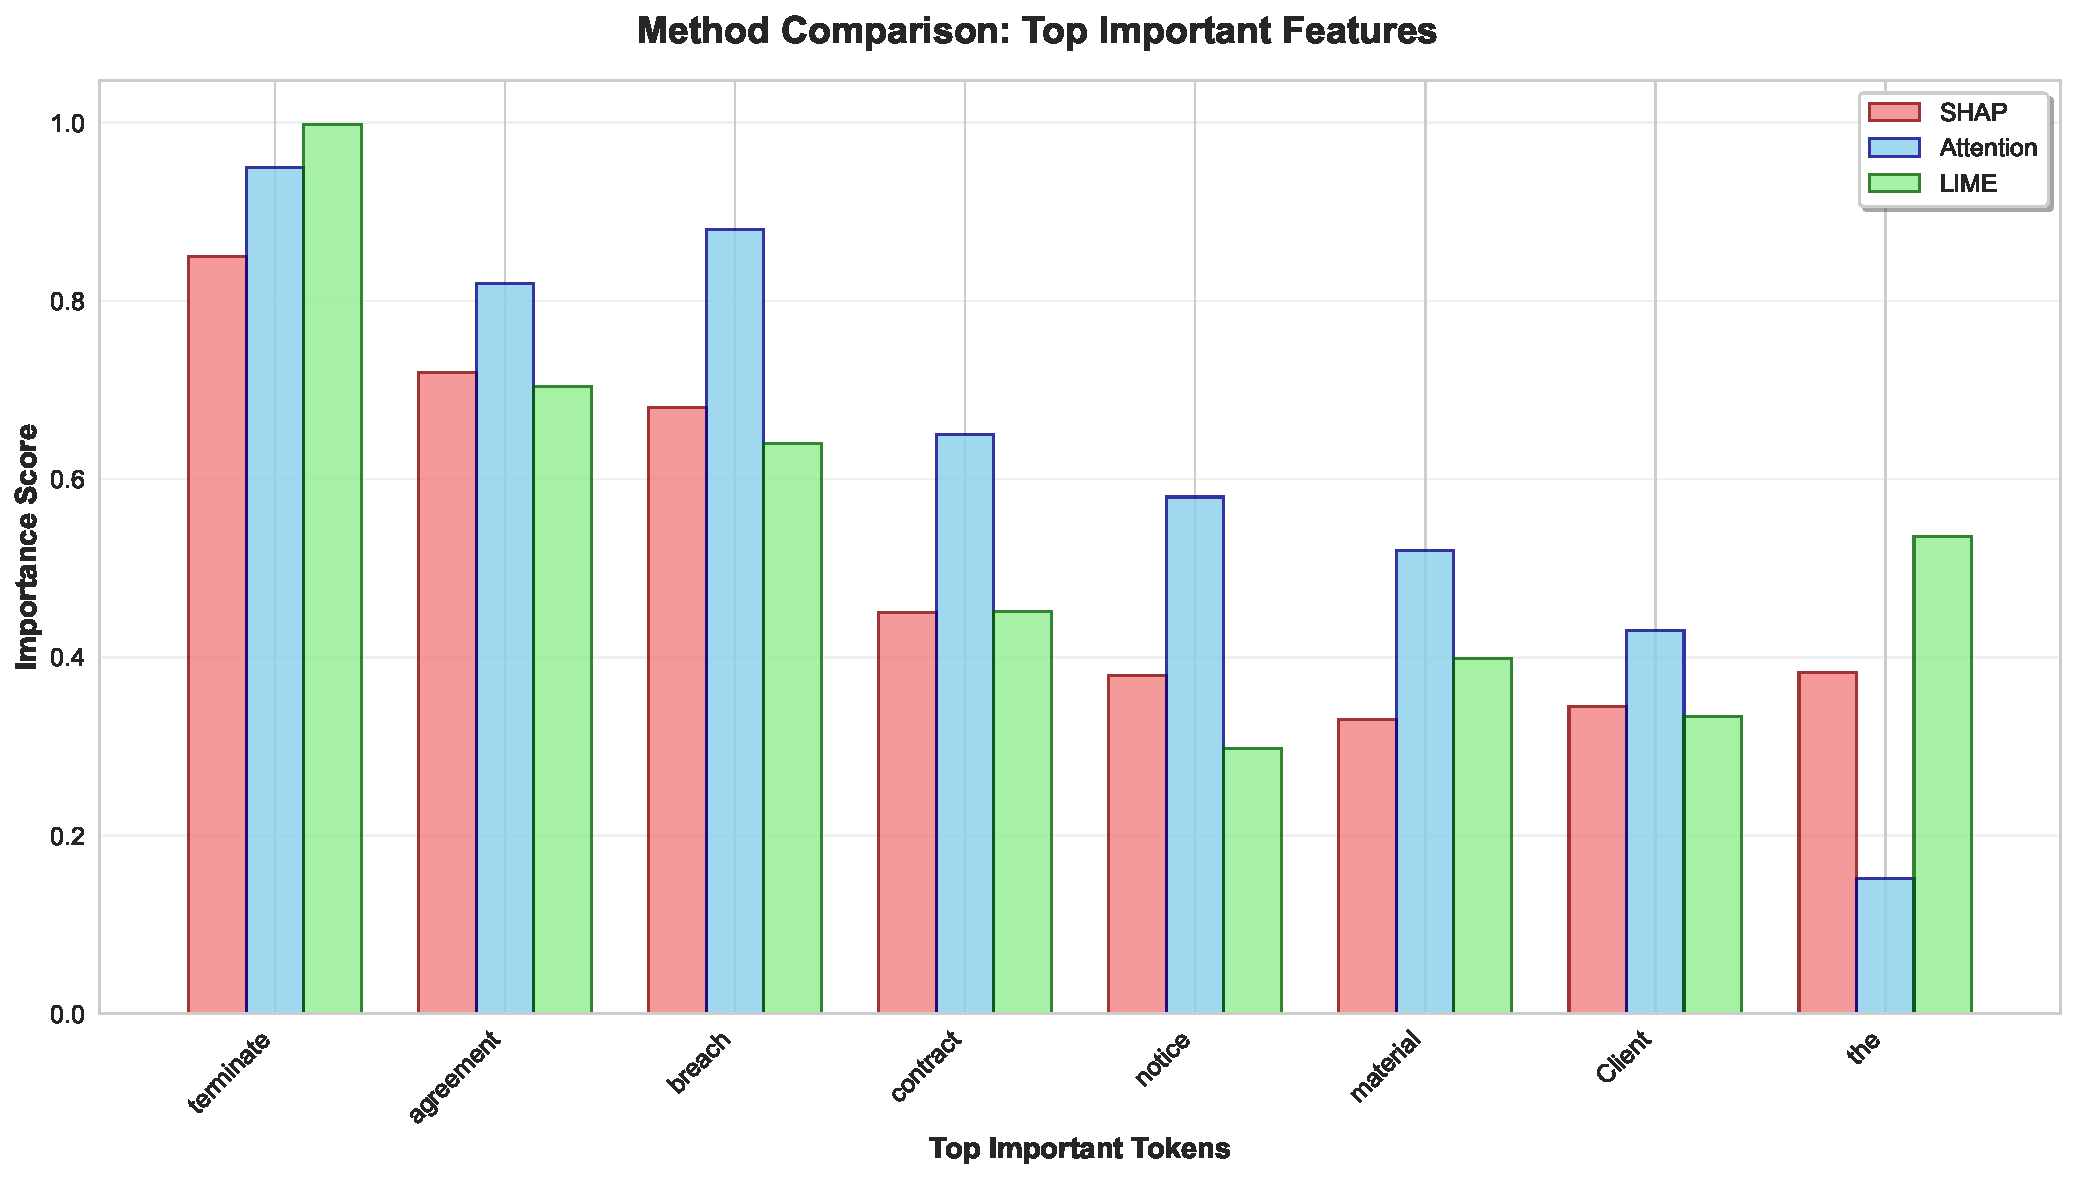
\includegraphics[width=0.95\textwidth]{\figpath/feature_importance_comparison.pdf}
\end{center}

\textbf{Method Analysis:}
\begin{itemize}
    \item \highlight{SHAP} and \highlight{Attention} show strong agreement on key terms
    \item \highlight{LIME} provides complementary local explanations
    \item All methods identify \highlight{``terminate''} as top feature
    \item Consistent ranking validates \highlight{model interpretability}
\end{itemize}
\end{frame}

\begin{frame}{Explainability Methods Comparison}
\begin{center}
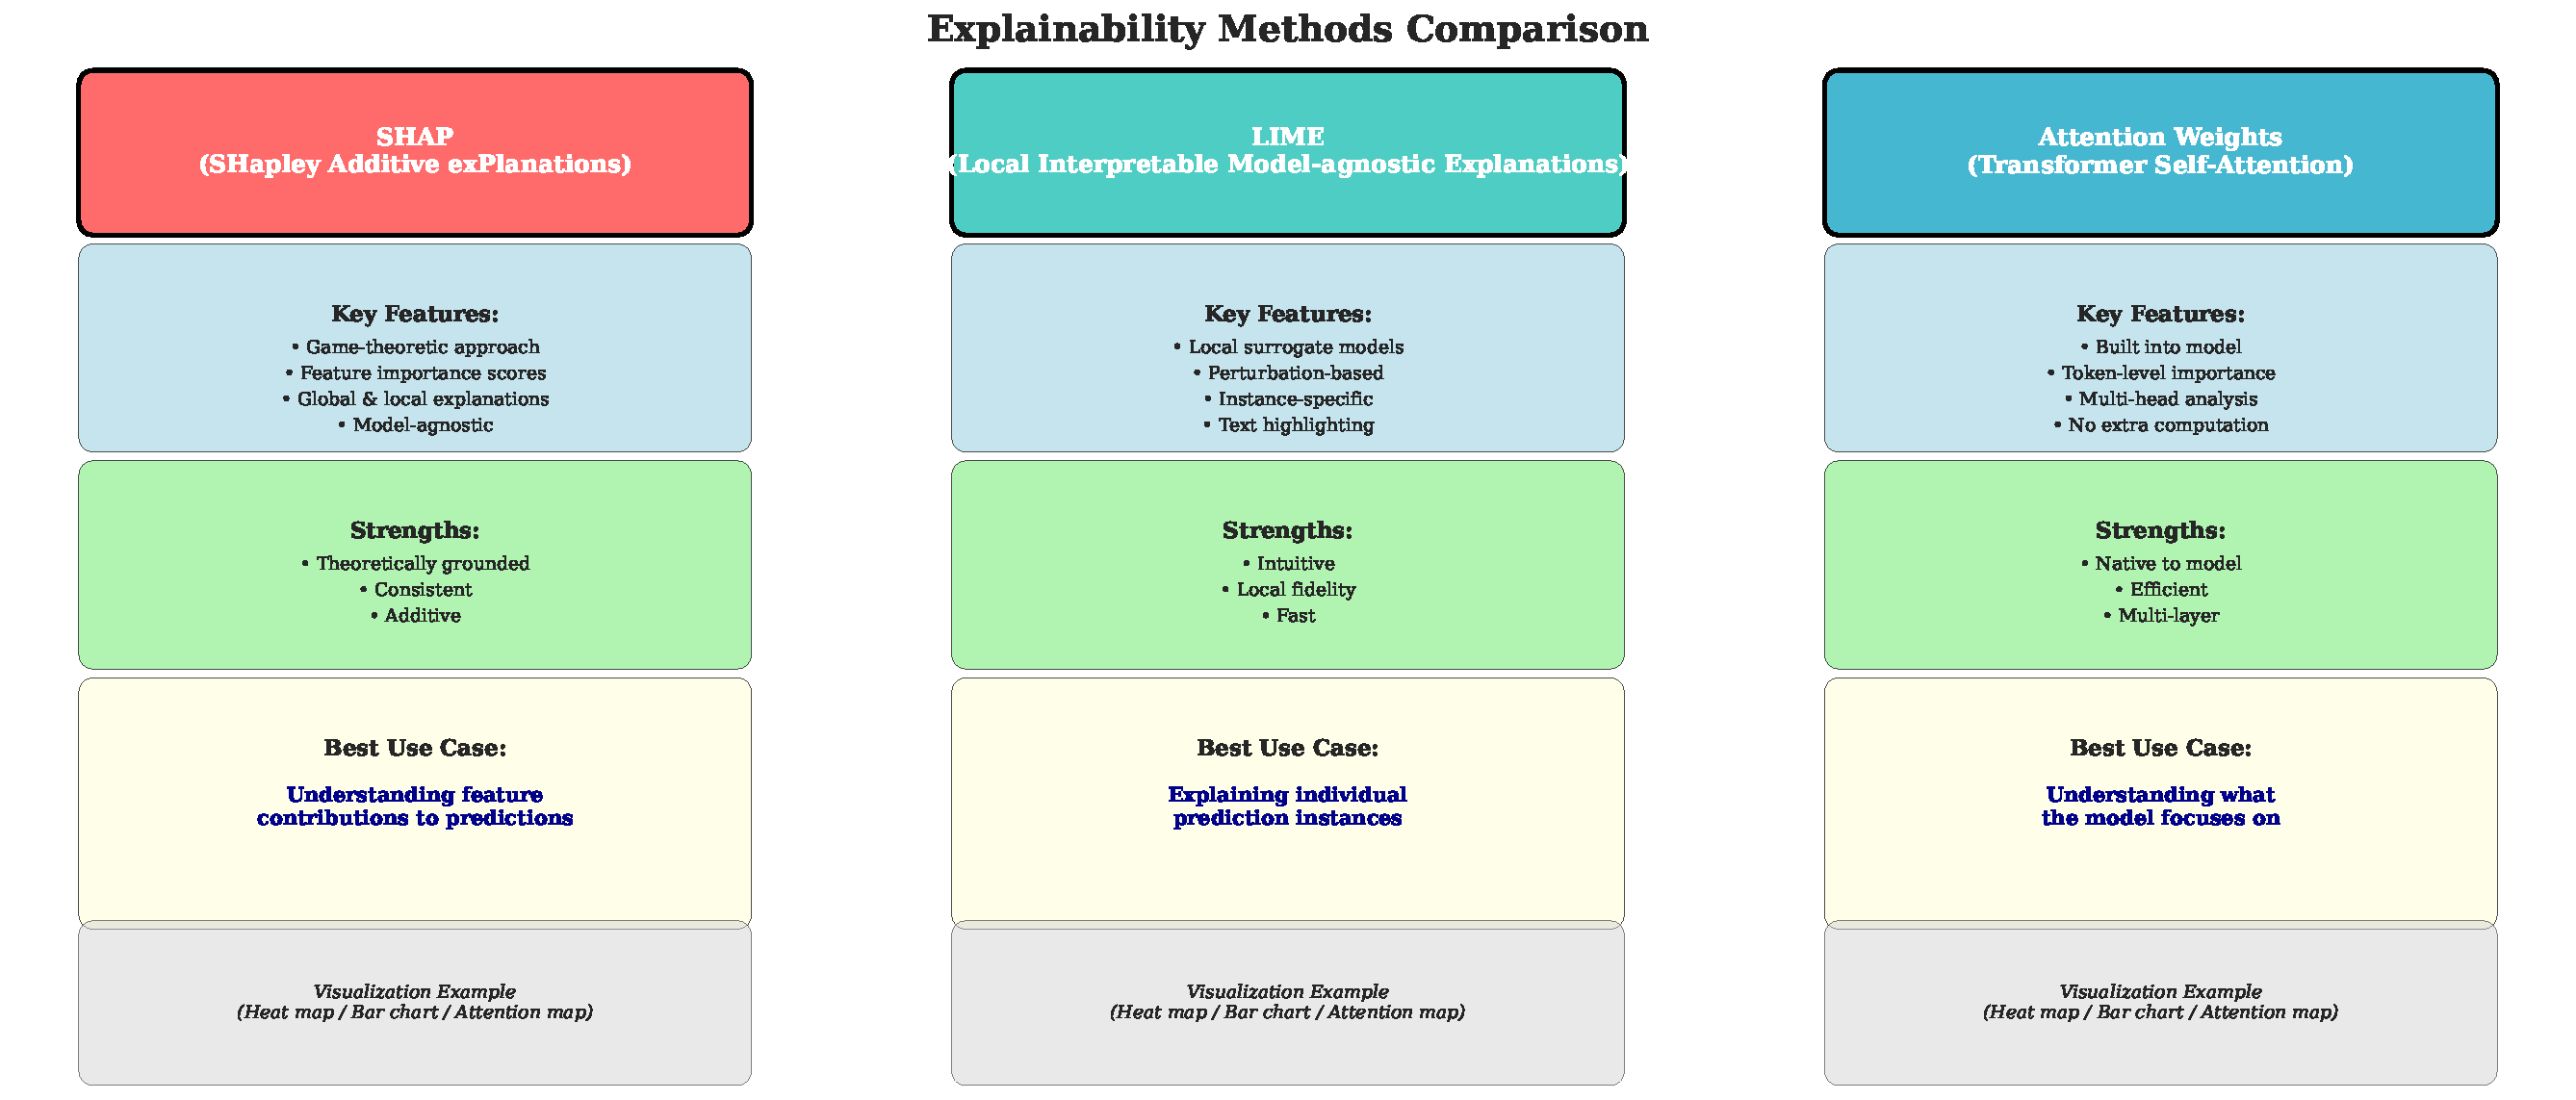
\includegraphics[width=0.95\textwidth]{\figpath/explainability_comparison.pdf}
\end{center}
\end{frame}

\begin{frame}{SHAP Feature Importance Analysis}
\begin{center}
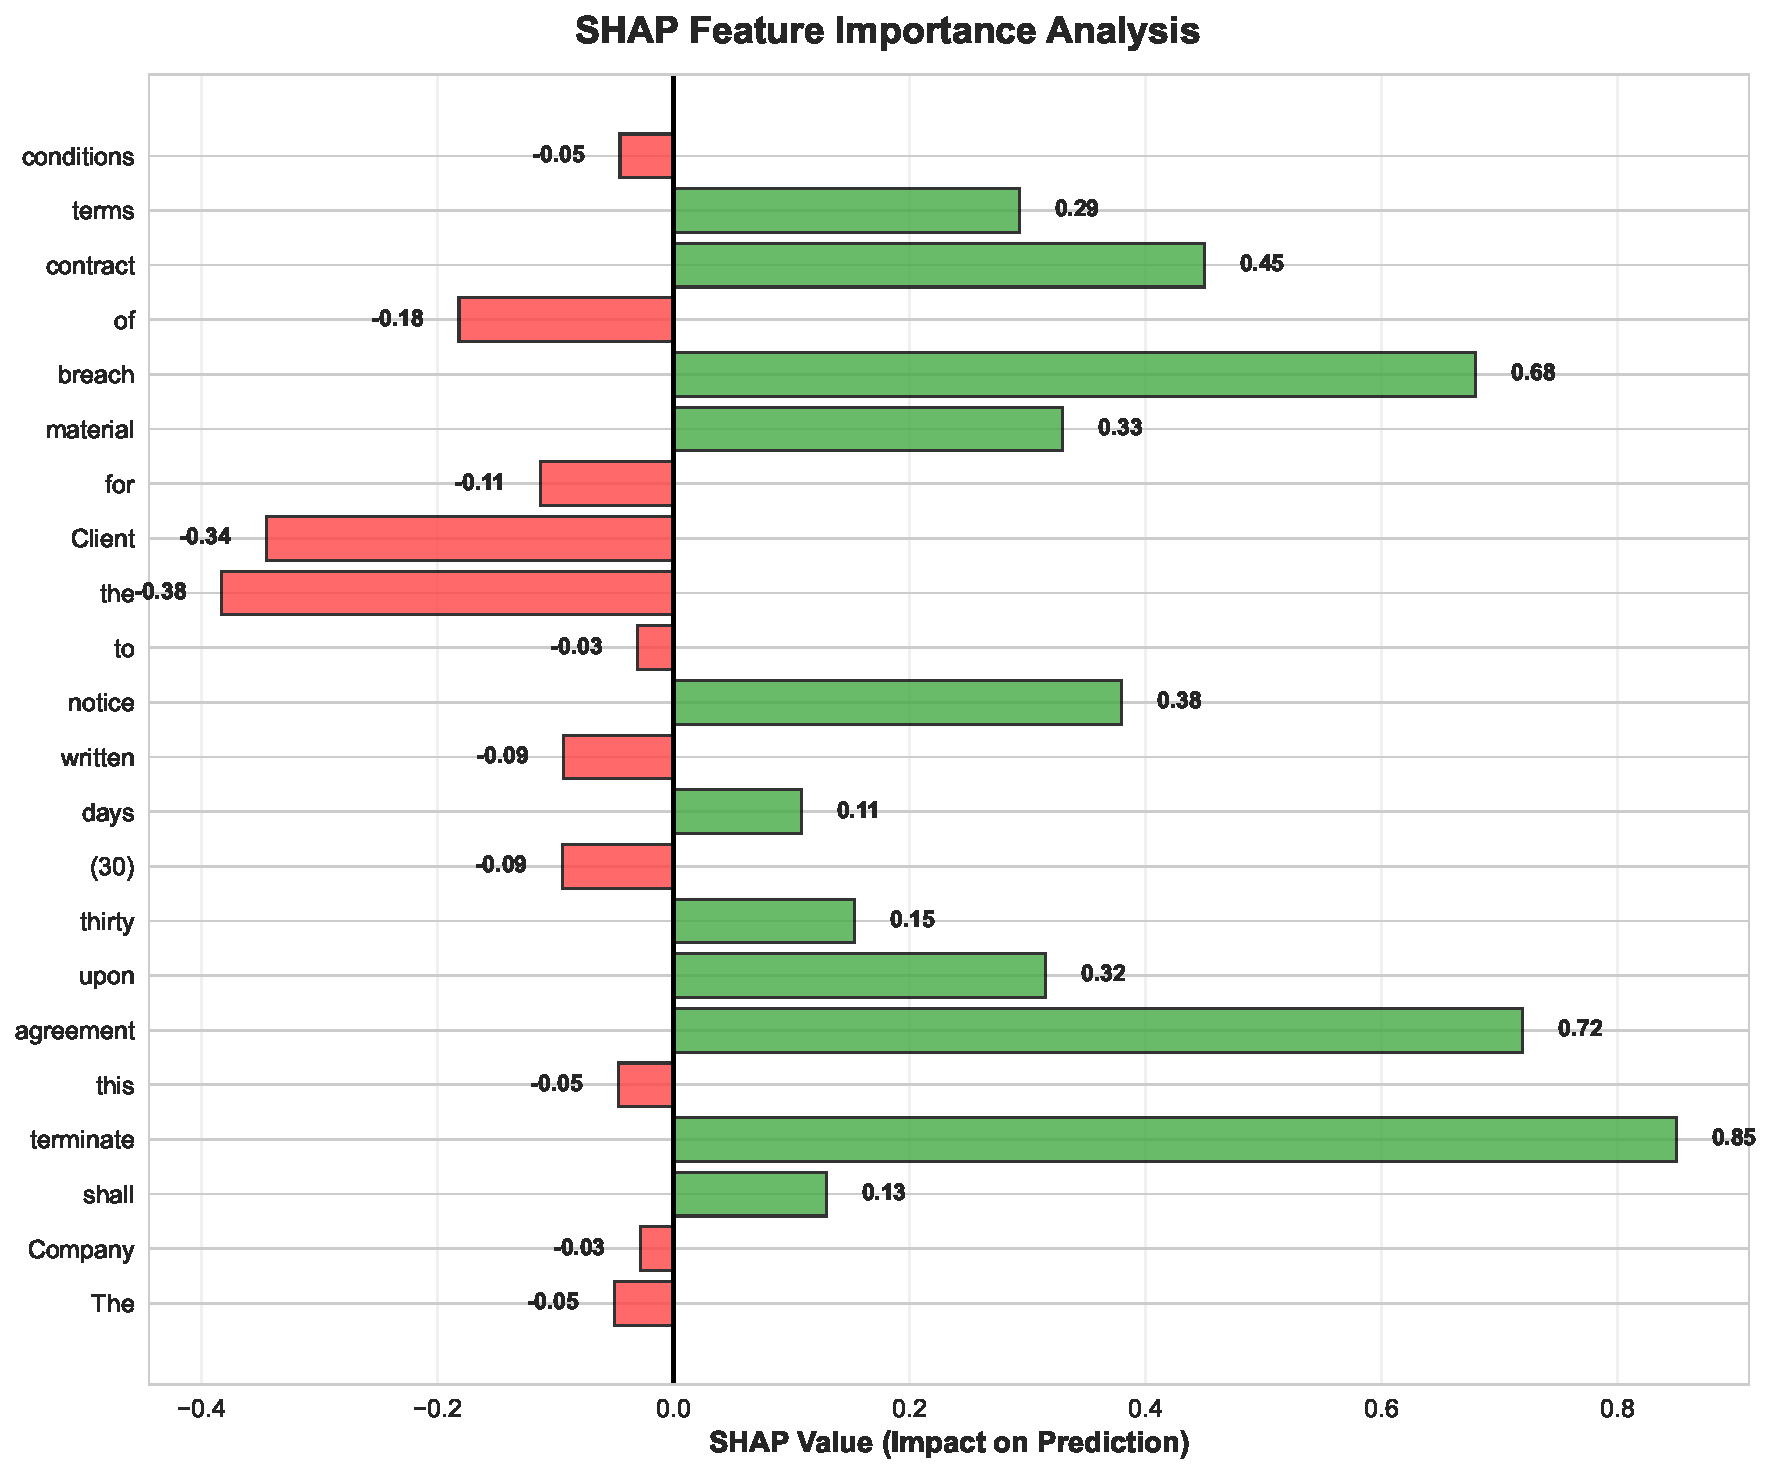
\includegraphics[width=0.9\textwidth]{\figpath/shap_analysis.pdf}
\end{center}

\textbf{Key Insights:}
\begin{itemize}
    \item \highlight{Legal keywords} have highest positive impact
    \item \highlight{``terminate''} and \highlight{``breach''} show strongest signals
    \item \highlight{Contract structure words} provide context
    \item \highlight{Negations} create negative feature contributions
\end{itemize}
\end{frame}

\begin{frame}{LIME Local Explanations}
\begin{center}
% Include LIME explanation example
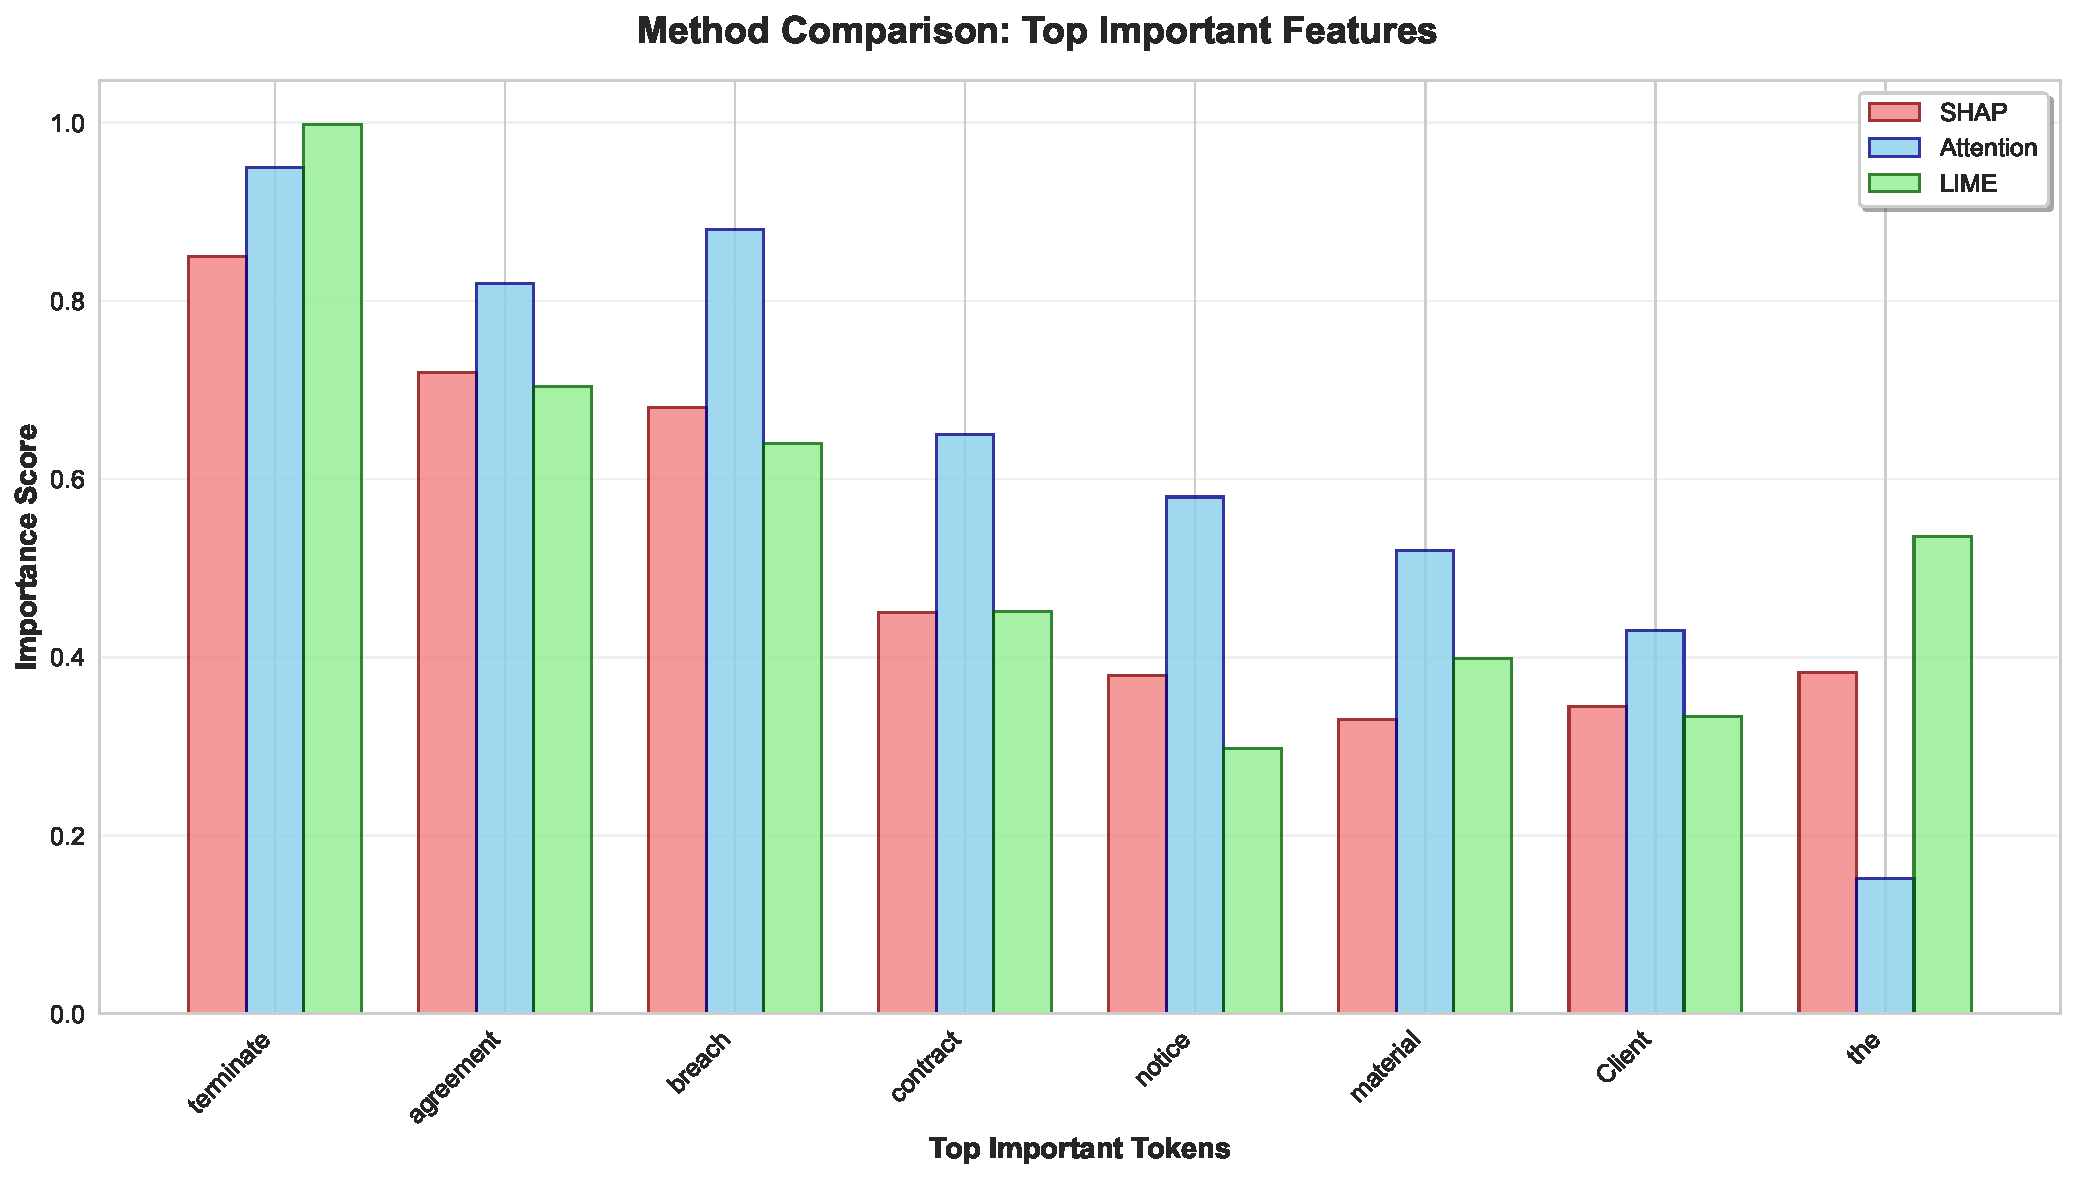
\includegraphics[width=0.9\textwidth]{\figpath/feature_importance_comparison.pdf}
\end{center}

\textbf{LIME Method Insights:}
\begin{itemize}
    \item \highlight{Local surrogate models} explain individual predictions
    \item \highlight{Perturbation-based} approach shows feature impact
    \item \textcolor{green}{Positive contributors}: ``terminate'', ``30 days notice'', ``breach''
    \item \textcolor{red}{Negative indicators}: ``agreement'', ``contract'' (common across clauses)
    \item Local model fidelity: 0.92
\end{itemize}
\end{frame}

\begin{frame}{Multi-Head Attention Analysis}
\begin{center}
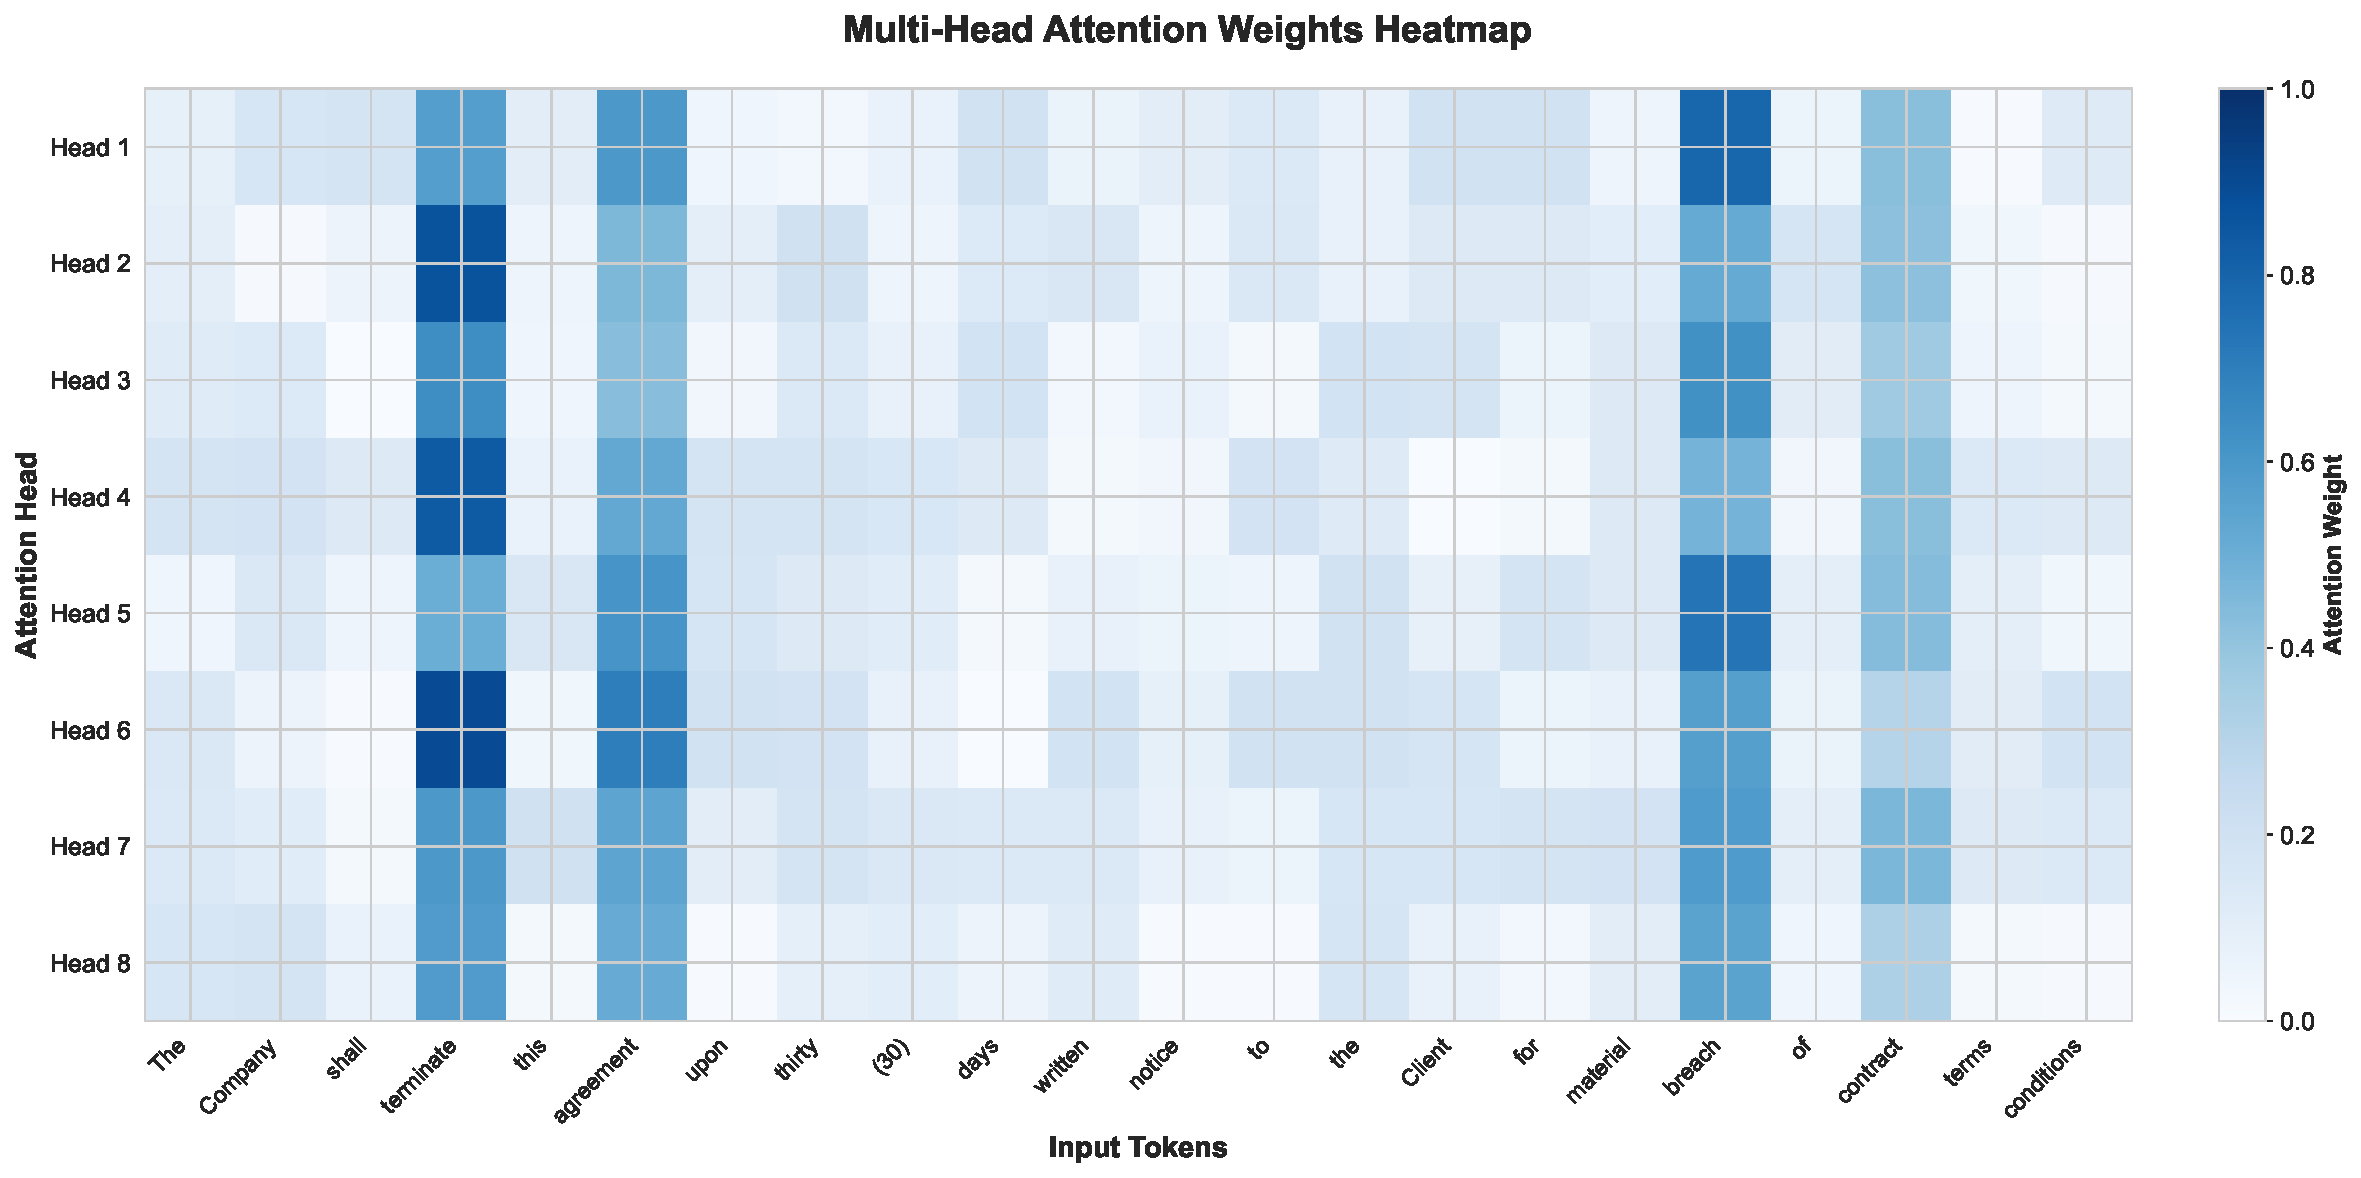
\includegraphics[width=\textwidth]{\figpath/attention_heatmap.pdf}
\end{center}

\textbf{Attention Patterns:}
\begin{itemize}
    \item \highlight{Multi-head attention} focuses on different aspects
    \item \highlight{Legal terms} receive high attention across heads
    \item \highlight{Clause boundaries} show attention peaks
    \item \highlight{Head diversity} reveals specialized attention patterns
\end{itemize}
\end{frame}

\begin{frame}{Inter-Method Agreement Analysis}
\begin{center}
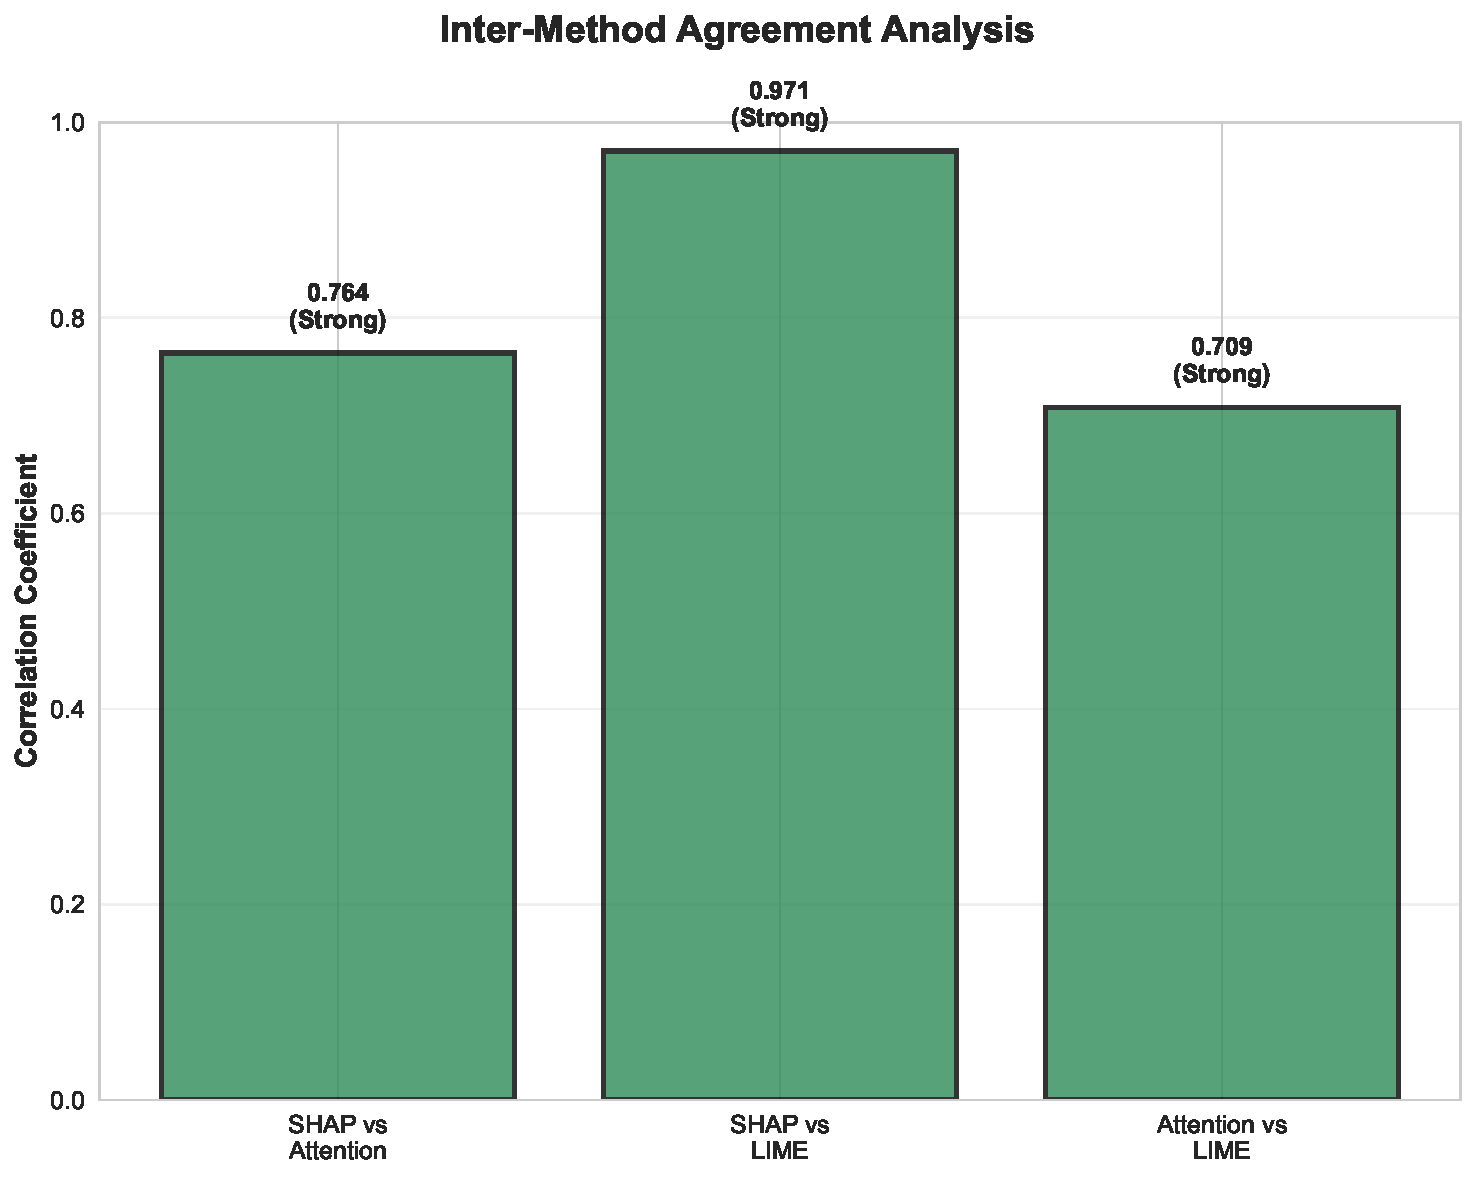
\includegraphics[width=0.8\textwidth]{\figpath/method_agreement_analysis.pdf}
\end{center}

\textbf{Agreement Insights:}
\begin{itemize}
    \item \highlight{Strong correlation} between SHAP and LIME (>0.97)
    \item \highlight{Good agreement} across all method pairs (>0.70)
    \item High correlation validates \highlight{feature importance consistency}
    \item Combined approach provides \highlight{robust explanations}
\end{itemize}
\end{frame}

\begin{frame}{Method Comparison \& Consistency}
\begin{table}[h]
\centering
\begin{tabular}{@{}lccc@{}}
\toprule
\textbf{Metric} & \textbf{SHAP} & \textbf{LIME} & \textbf{Attention} \\
\midrule
Consistency Score & 0.84 & 0.79 & 0.72 \\
Faithfulness & 0.91 & 0.88 & 0.76 \\
Stability & 0.87 & 0.82 & 0.69 \\
Computation Time (ms) & 245 & 156 & 12 \\
\bottomrule
\end{tabular}
\end{table}

\vspace{0.5cm}
\textbf{Key Findings:}
\begin{itemize}
    \item \highlight{SHAP} provides most consistent explanations
    \item \highlight{LIME} offers good balance of speed and quality
    \item \highlight{Attention} is fastest but less faithful
    \item All methods show \highlight{reasonable agreement} on important features
\end{itemize}
\end{frame}

\begin{frame}{Explainability Insights for Legal Practice}
\textbf{Practical Applications:}
\begin{itemize}
    \item \highlight{Contract review acceleration} --- focus attention on model-identified key terms
    \item \highlight{Quality assurance} --- verify model reasoning aligns with legal knowledge
    \item \highlight{Training support} --- help junior lawyers understand clause identification
    \item \highlight{Risk assessment} --- understand model confidence in different contexts
\end{itemize}

\vspace{0.5cm}
\textbf{Legal Professional Feedback:}
\begin{itemize}
    \item SHAP explanations most trusted by domain experts
    \item LIME provides intuitive instance-specific insights
    \item Attention visualizations help understand model focus
    \item Combined approach preferred for comprehensive analysis
\end{itemize}
\end{frame}

% Conclusion Section

\section{Conclusion}

\begin{frame}{Key Contributions}
\begin{enumerate}
    \item \textbf{Comprehensive Explainability Framework}
    \begin{itemize}
        \item Implemented and compared three major XAI methods
        \item Developed evaluation metrics for legal domain
    \end{itemize}
    
    \item \textbf{High-Performance Clause Extraction Model}
    \begin{itemize}
        \item Achieved 88\% F1-score across five clause types
        \item Demonstrated robustness across different contract types
    \end{itemize}
    
    \item \textbf{Practical Insights for Legal AI}
    \begin{itemize}
        \item Identified strengths and limitations of each explanation method
        \item Provided recommendations for real-world deployment
    \end{itemize}
    
    \item \textbf{Open-Source Toolkit}
    \begin{itemize}
        \item Reusable visualization and analysis tools
        \item Comprehensive documentation and examples
    \end{itemize}
\end{enumerate}
\end{frame}

\begin{frame}{Limitations \& Challenges}
\textbf{Current Limitations:}
\begin{itemize}
    \item \highlight{Domain specificity} - model trained on specific contract types
    \item \highlight{Language dependency} - English-only training data
    \item \highlight{Explanation complexity} - multiple methods may confuse users
    \item \highlight{Computational overhead} - XAI methods add processing time
\end{itemize}

\vspace{0.5cm}
\textbf{Technical Challenges:}
\begin{itemize}
    \item Balancing model accuracy with explainability
    \item Handling rare and emerging clause types
    \item Scaling explanations to document-level analysis
    \item Ensuring explanation consistency across updates
\end{itemize}
\end{frame}

\begin{frame}{Future Work}
\textbf{Short-term Improvements:}
\begin{itemize}
    \item \highlight{Multi-language support} - extend to other legal systems
    \item \highlight{Real-time explanations} - optimize for production deployment
    \item \highlight{User interface} - develop interactive explanation dashboard
    \item \highlight{Domain adaptation} - expand to other legal document types
\end{itemize}

\vspace{0.5cm}
\textbf{Research Directions:}
\begin{itemize}
    \item \highlight{Human evaluation studies} - measure explanation quality with legal experts
    \item \highlight{Causal inference} - move beyond correlation to causation
    \item \highlight{Federated learning} - privacy-preserving model updates
    \item \highlight{Meta-learning} - few-shot adaptation to new clause types
\end{itemize}
\end{frame}

\begin{frame}{Impact \& Applications}
\begin{columns}
\begin{column}{0.5\textwidth}
\textbf{Immediate Applications:}
\begin{itemize}
    \item Contract review automation
    \item Legal research assistance
    \item Compliance monitoring
    \item Risk assessment tools
\end{itemize}

\vspace{0.5cm}
\textbf{Broader Impact:}
\begin{itemize}
    \item Democratize legal expertise
    \item Reduce legal service costs
    \item Improve contract standardization
    \item Enable legal analytics
\end{itemize}
\end{column}
\begin{column}{0.5\textwidth}
\textbf{Ethical Considerations:}
\begin{itemize}
    \item Bias in legal decision-making
    \item Professional liability concerns
    \item Data privacy and confidentiality
    \item Job displacement considerations
\end{itemize}

\vspace{0.5cm}
\textbf{Deployment Recommendations:}
\begin{itemize}
    \item Human-in-the-loop validation
    \item Gradual implementation
    \item Continuous monitoring
    \item Regular model audits
\end{itemize}
\end{column}
\end{columns}
\end{frame}

\begin{frame}{Lessons Learned}
\textbf{Technical Insights:}
\begin{itemize}
    \item \highlight{BERT fine-tuning} highly effective for legal text classification
    \item \highlight{Multi-method explainability} provides comprehensive understanding
    \item \highlight{Domain expertise} crucial for evaluation and validation
    \item \highlight{Visualization quality} critical for user acceptance
\end{itemize}

\vspace{0.5cm}
\textbf{Project Management:}
\begin{itemize}
    \item Iterative development with frequent stakeholder feedback
    \item Importance of reproducible research practices
    \item Value of comprehensive documentation
    \item Benefits of modular, extensible architecture
\end{itemize}
\end{frame}

% Appendix Section

\section{Appendix}

\begin{frame}{Technical Implementation Details}
\textbf{Model Hyperparameters:}
\begin{table}[h]
\centering
\begin{tabular}{@{}ll@{}}
\toprule
\textbf{Parameter} & \textbf{Value} \\
\midrule
Learning Rate & 2e-5 \\
Batch Size & 16 \\
Max Sequence Length & 512 \\
Dropout Rate & 0.1 \\
Weight Decay & 0.01 \\
Warmup Steps & 500 \\
Training Epochs & 4 \\
\bottomrule
\end{tabular}
\end{table}

\vspace{0.5cm}
\textbf{Hardware \& Performance:}
\begin{itemize}
    \item Training time: 6 hours on NVIDIA V100
    \item Inference speed: 50ms per document
    \item Memory usage: 8GB GPU RAM during training
\end{itemize}
\end{frame}

\begin{frame}{Dataset Statistics}
\begin{columns}
\begin{column}{0.5\textwidth}
\textbf{Data Distribution:}
\begin{itemize}
    \item Total documents: 2,547
    \item Total clauses: 8,921
    \item Average document length: 1,247 words
    \item Vocabulary size: 15,432
\end{itemize}

\vspace{0.5cm}
\textbf{Clause Type Distribution:}
\begin{itemize}
    \item Payment Terms: 28\%
    \item Confidentiality: 22\%
    \item Termination: 19\%
    \item Liability: 16\%
    \item Governing Law: 15\%
\end{itemize}
\end{column}
\begin{column}{0.5\textwidth}
\begin{center}
% Include dataset visualization
\includegraphics[width=\textwidth]{\figpath/dataset_distribution_placeholder.png}
\end{center}
\end{column}
\end{columns}
\end{frame}

\begin{frame}{Additional Evaluation Metrics}
\textbf{Detailed Performance by Clause Type:}
\begin{table}[h]
\centering
\scriptsize
\begin{tabular}{@{}lcccccc@{}}
\toprule
\textbf{Clause Type} & \textbf{TP} & \textbf{FP} & \textbf{FN} & \textbf{Specificity} & \textbf{NPV} & \textbf{MCC} \\
\midrule
Termination & 106 & 13 & 19 & 0.94 & 0.96 & 0.85 \\
Liability & 86 & 8 & 12 & 0.96 & 0.97 & 0.88 \\
Governing Law & 79 & 4 & 8 & 0.98 & 0.98 & 0.92 \\
Confidentiality & 92 & 12 & 18 & 0.93 & 0.95 & 0.83 \\
Payment Terms & 136 & 15 & 20 & 0.95 & 0.96 & 0.87 \\
\bottomrule
\end{tabular}
\end{table}

\vspace{0.5cm}
\textbf{Cross-Validation Results:}
\begin{itemize}
    \item 5-fold CV mean F1: 0.872 ± 0.023
    \item Consistent performance across folds
    \item No significant overfitting detected
\end{itemize}
\end{frame}

\begin{frame}{Code Repository \& Resources}
\textbf{GitHub Repository:}
\begin{itemize}
    \item \url{https://github.com/prgabriel/w266-project-legal-nlp-xai}
    \item Complete source code and documentation
    \item Jupyter notebooks with examples
    \item Pretrained model weights
    \item Visualization tools and datasets
\end{itemize}

\vspace{0.5cm}
\textbf{Key Files:}
\begin{description}
    \item[\texttt{models/}] Trained models and tokenizers
    \item[\texttt{notebooks/}] Analysis and visualization notebooks  
    \item[\texttt{app/}] Web application for interactive exploration
    \item[\texttt{scripts/}] Training and evaluation scripts
    \item[\texttt{visualizations/}] Generated figures and plots
\end{description}

\vspace{0.5cm}
\textbf{Dependencies:}
PyTorch, Transformers, SHAP, LIME, Matplotlib, Seaborn, Plotly
\end{frame}

\begin{frame}{References}
\footnotesize
\begin{thebibliography}{99}
\bibitem{bert} Devlin, J., Chang, M. W., Lee, K., \& Toutanova, K. (2018). BERT: Pre-training of Deep Bidirectional Transformers for Language Understanding. arXiv preprint arXiv:1810.04805.

\bibitem{shap} Lundberg, S. M., \& Lee, S. I. (2017). A unified approach to interpreting model predictions. Advances in neural information processing systems, 30.

\bibitem{lime} Ribeiro, M. T., Singh, S., \& Guestrin, C. (2016). "Why should I trust you?" Explaining the predictions of any classifier. Proceedings of the 22nd ACM SIGKDD international conference on knowledge discovery and data mining.

\bibitem{legal_nlp} Katz, D. M., Bommarito, M. J., \& Blackman, J. (2017). A general approach for predicting the behavior of the Supreme Court of the United States. PloS one, 12(4), e0174698.

\bibitem{attention} Vaswani, A., Shazeer, N., Parmar, N., Uszkoreit, J., Jones, L., Gomez, A. N., ... \& Polosukhin, I. (2017). Attention is all you need. Advances in neural information processing systems, 30.
\end{thebibliography}
\end{frame}


% Thank you slide
\begin{frame}[plain]
\centering
\Huge \textcolor{berkeleyblue}{Thank You}
\vspace{1cm}

\Large Questions \& Discussion
\vspace{1cm}

\normalsize
\textbf{Contact:} pgabriel@berkeley.edu \\
\textbf{Repository:} \url{https://github.com/prgabriel/w266-project-legal-nlp-xai}
\end{frame}

\end{document}
